%    Copyright (C) Adapted Version by Tiefenbacher (philipp.tiefenbacher@tum.de)
% 	 Original version from Moritz Kaiser
%    Institute for Human-Machine Communication
%    Technische Universität München, Germany
%    
%
%    %%%%%%%%%%%%%%%%%%%%%%%%%%%%%%%%%%%%%%%%%%%%%%%%%%%%%%%%%%%%%
%    Document:       Template for master's thesis at our institute
%    Version:        0.5
%    %%%%%%%%%%%%%%%%%%%%%%%%%%%%%%%%%%%%%%%%%%%%%%%%%%%%%%%%%%%%%

\documentclass{mmkthesis} %set to mmkthesis_deutsch when writing in german

%%%%%%%%%%%%%%%%%%%%%%%%%%%%%%%%%%%%%%%%%%%%%%%%%%%%%%%
% Include packages, these are only the basic packages %
% Add own things if you want                          %
%%%%%%%%%%%%%%%%%%%%%%%%%%%%%%%%%%%%%%%%%%%%%%%%%%%%%%%

\usepackage[german, english]{babel}               
% We want to have some math
\usepackage{amsmath}
% For the set of real numbers
\usepackage{amsfonts}
% Nice figures
\usepackage{graphicx}
% with subfigures
\usepackage[tight]{subfigure}
% Wrap text around figures
\usepackage{wrapfig}    
% More beautiful tables
\usepackage{booktabs}
% For pseudo codes (don't forget the noend option)
\usepackage{algorithmic}
\usepackage{algorithm}

%create nice graphics with tikz. We recommend to convert your matlab plots with matlab2tikz to a tikz file.
%\usepackage{tikz}
%\usepackage{pgfplots}
%\usetikzlibrary{external, arrows, scopes, decorations.pathreplacing, shapes.geometric, matrix, positioning, decorations.markings}

%convert eps to pdf --> faster compilation of document
%\usepackage{epstopdf}

%extended enumeration environemt, e.g., inline enumerations
%\usepackage{enumitem}

%want to read and revise your printed document. Use double space to have more space for corrections between lines.
%\usepackage{setspace}
%\doublespacing

%more beautiful fractions
%\usepackage{nicefrac}

%you want to add an url?
\usepackage{url}

% Make overfull errors more visible in the output PDF by setting \overfullrule:
\overfullrule=1pt

% Own commands - very helpful
% \input frontmatter/newcommands.tex


%%%%%%%%%%%%%%%%%%%%%%%%%%%%%%%%%%%%%%%%%%
% Document information for the titlepage %
%%%%%%%%%%%%%%%%%%%%%%%%%%%%%%%%%%%%%%%%%%
\newcommand{\mmktitle}{Development of a Description\\\vspace{0.1cm} % Title of the thesis
            Format for Road System Generated\\\vspace{0.2cm}  		% add vspace if your title
     		by SUMO and City Engine for MMK Car Simulator}          % does not occupy three lines
\newcommand{\mmkauthor}{Zhechko Zhechev}                            % You, the author, no plagiarism
\newcommand{\mmkadvisor}{Patrick Lindemann, M.Sc.}          			% Your advisor
				%in case of a B.Sc. or M.Sc title: NameOfYou/YourAdvisor, B.Sc.
\newcommand{\mmktypeofwork}{IDP Final Report}                        % Bachelor/Master/IDP, etc.        
\newcommand{\startedon}{30.04.2016}                                 % Started on
\newcommand{\handedinon}{15.12.2017}                                % Handed in on

\begin{document}
%%%%%%%%%%%
%if you write in german, uncomment the next line
%\selectlanguage{german}   
%%%%%%%%%%%

\titlepage    % The TUM typical title page, defined in the mmkthesis class
%%%%%%%%%%%%%%%%%%%%%%%%%%%%%%%%%%%%%%%%%%%%%%%%%%%%%%%%%%%%%%%%%%%%%%%%
% Frontmatter, usually incorporates acknowledgements and abstract, see %
%             http://en.wikipedia.org/wiki/Book_design                 %
%%%%%%%%%%%%%%%%%%%%%%%%%%%%%%%%%%%%%%%%%%%%%%%%%%%%%%%%%%%%%%%%%%%%%%%%   
% \frontmatter, \mainmatter, \backmatter is for the book class
\frontmatter
\chapter*{Abstract}



\tableofcontents

%%%%%%%%%%%%%%
% Mainmatter %
%%%%%%%%%%%%%%
\mainmatter
% Introduction
\chapter{Introduction}
\label{ch:introduction}
% Mixed Reality-Driving Simulator developed using Unity 3D-Engine 
Augmented reality has not only changed the perception of the world for the ordinary user but it has also allowed researchers to conduct studies which have not been possible before. The chair of Human Machine Communication is currently developing a mixed reality driving simulator using Unity Engine in a 3D CAVE. It can be utilised to facilitate studies regarding reaction of the driver in different situations on the road and development of better Head-Up Displays.

Currently, the 3D models which simulate the street network are generated using ESRI CityEngine and unfortunately, they are not based on real data. Moreover, a semantic description of the underlaying street network, as well as any properties of its segment are not present. Street information based on real data exported from open source projects such as OpenStreetMap would improve the quality of the generated models. This would allow the simulation of real scenes and furthermore facilitate the research of the human-machine interaction. Additionally, a semantic description of the street network would allow the simulation of autonomous vehicles and fully simulation of traffic management system. 
 
\section{Goals of the Project}
\label{sec:goals}
The main goal of this Interdisciplinary Project is to derive semantic description of the road network, generated using OpenStreetMap data in CityEngine and SUMO. Moreover, the generated 3D scene of a city model has to be synchronised with the aforementioned description. Additionally, the export document has to contain all details about the lanes which compose all corresponding road segments and their properties, as well as the coordinates of buildings and parkings which can be found in the generated scene. The export must be accomplished in a widely compatible format which has proven suitable for these purposes, as well. Finally, the road network description has to be imported in the MMK Driving Simulator in order to build a navigation system for the traffic participants using the already generated connectivity information by SUMO.

\section{Outline}
\label{sec:outline}
The remainder of this report is organised as follows: Chapter \ref{ch:background} provides background information about the essential tools which are used to improve the current functionalities of the MMK Driving Simulator. Later, in Chapter \ref{ch:descriptionOfRoadSystems}, we describe thoroughly our approach to derive a semantic description of the road system generated in CityEngine from OpenStreetMap data. Moreover, we discuss how additional road information can be derived from SUMO simulation files about the same road system. Afterwards, Chapter \ref{ch:gps} presents how we can furthermore utilise the SUMO-generated road connectivity information to construct a navigation system. Finally, Chapter \ref{ch:conclusion} makes a summary of the achieved goals and discusses possibilities for future improvements of the project.

%\begin{figure}[htb]
%	\centering
%	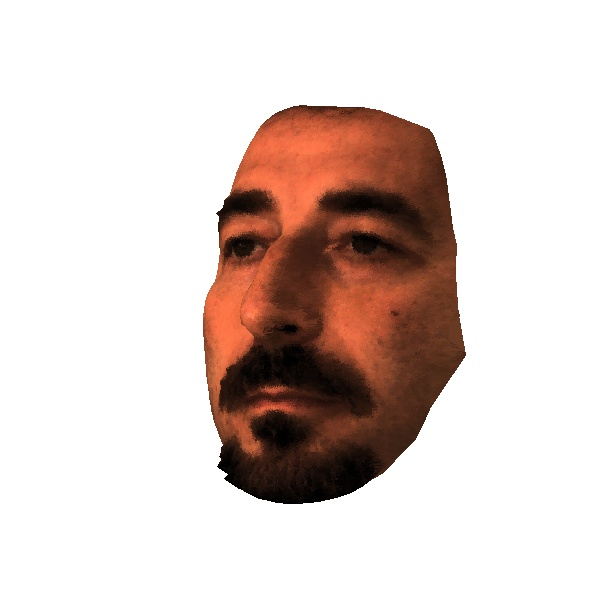
\includegraphics[width=0.35\linewidth]{figures/figure}
%	\caption{Some sample figure.}
%	\label{fig:sample}
%\end{figure}

% Background
\chapter{Background}
\label{ch:background}

% Coordinate Systems
\section{OpenStreetMap}
\label{ch:osm}

\section{ESRI City Engine}
\label{ch:ce}

\section{Simulation of Urban MObility (SUMO)}
\label{ch:sumo}

\section{Unity}
\label{ch:unity}

% Own work
\chapter{Semantic Description of Road Systems}
\label{ch:descriptionOfRoadSystems}
The following chapter provides a thorough description of the models and semantic description generation process for an urban aria from ESRI CityEngine (CE) using data provided by OpenStreetMap (OSM) combined in the end with SUMO simulation information. Moreover, we provide a detailed explanation of the resulting JSON format which holds data about essential scene objects. Lastly, we explain how the resulting file is parsed and used by Unity. Additionally, we defend design decisions, as well as describe failed attempts in the process.

A general overview of the whole process can be seen in Figure~\ref{fig:overview}. Firstly, OSM data of a given area is sanitised and imported in CE. The same sanitised data is provided to SUMO, which generates additional road details which are not present in CE. Afterwards, 3D models are generated together with the combined from CE and SUMO semantic road description data. In the end, they are imported and utilised in Unity. The navigation module which can be seen in \emph{Unity Game Engine} will be discussed in Chapter~\ref{ch:gps}.

\begin{figure}[htb]
	\centering
	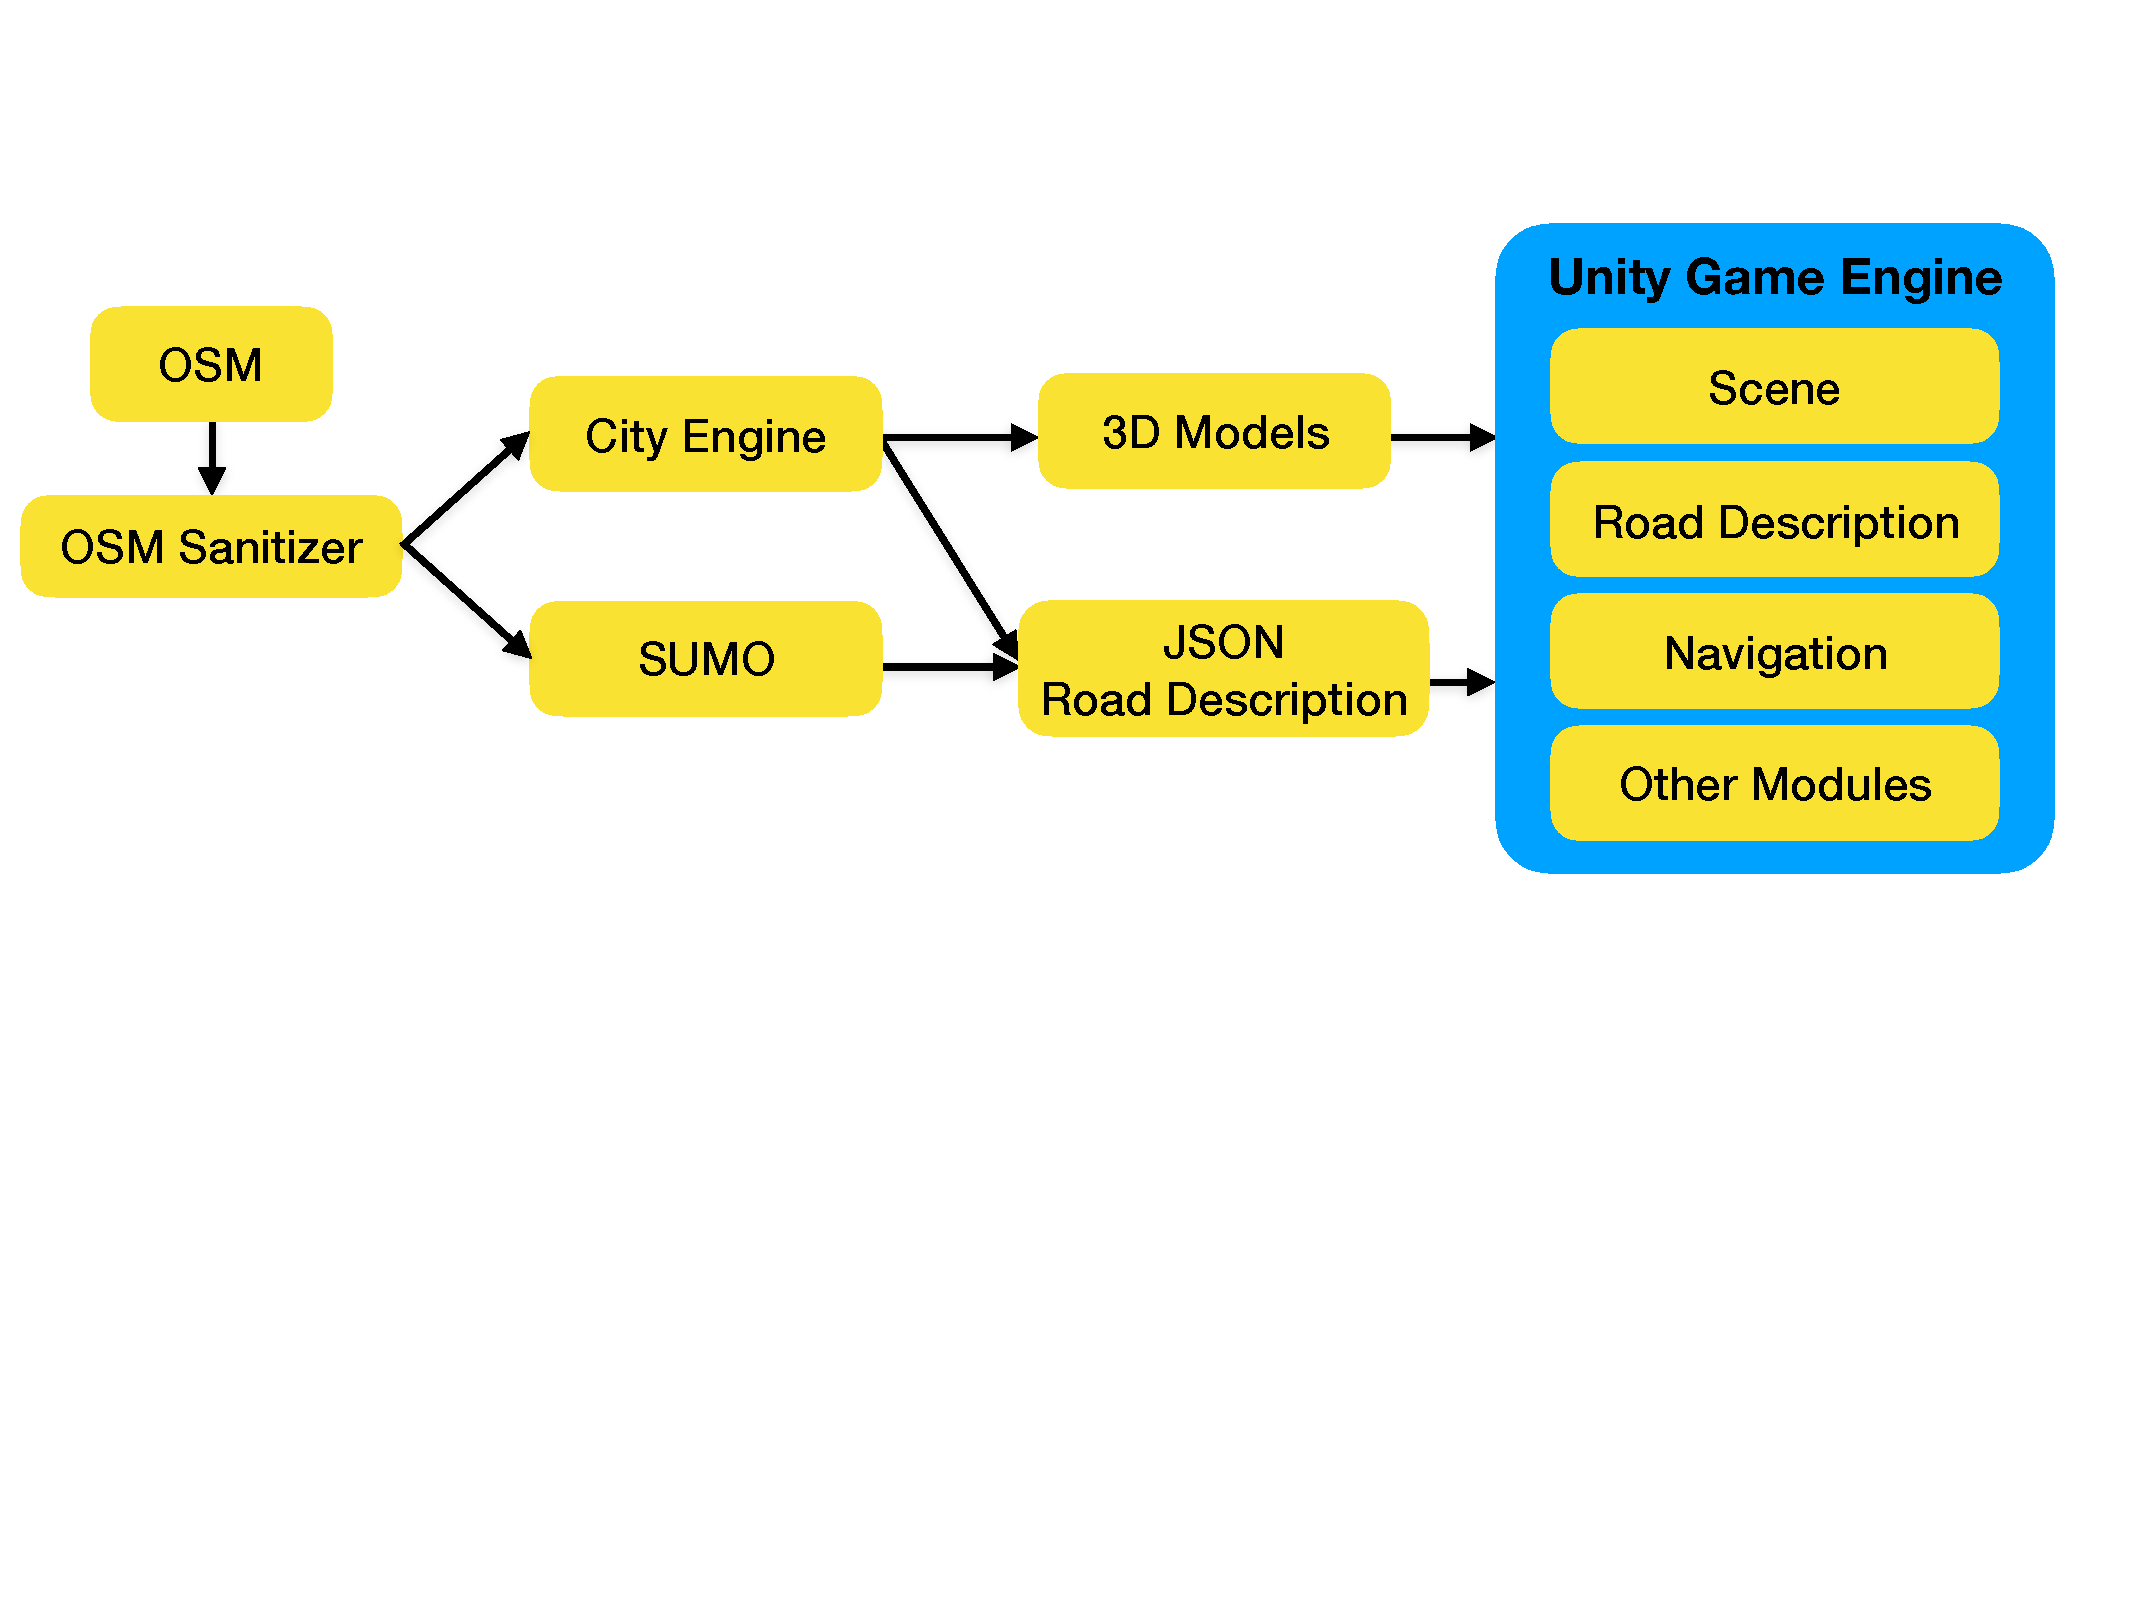
\includegraphics[width=0.95\linewidth]{figures/overview}
	\caption{Overview of the scene creation workflow.}
	\label{fig:overview}
\end{figure}

\section{OSM Export}
As already introduced, the whole map data used in the MMK Driving Simulator is exported from OSM. In Figure~\ref{fig:overview} we can see that exported \emph{OSM} file is given to the \emph{OSM Sanitizer} script, which removes some of the data in it. There are multiple reasons why this is necessary. Firstly, the objects contained in the export include some unnecessary information which is not utilised in the simulation, \emph{e.g.} underground network, footpaths. Moreover, this additional objects in the map represent an obstacle for both SUMO and CE in the scene generation process. For example, in Figure~\ref{fig:nosimply} and~\ref{fig:simply} one could see the difference in the shape creation between respectively an unsanitised and a sanitised version of the same \emph{OSM} export data.  

\begin{figure}[htb]
	\centering
	\subfigure[Unsanitised] {
	  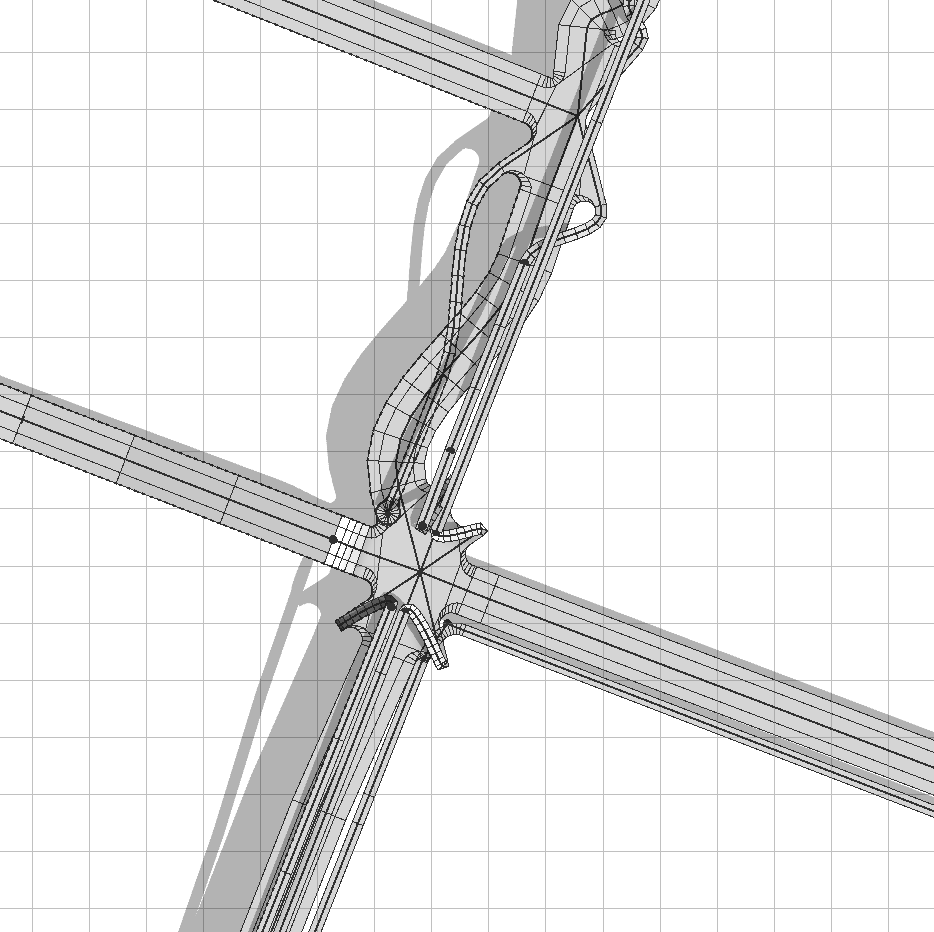
\includegraphics[width=0.4\textwidth]{figures/no-simply}
	  \label{fig:nosimply}
	}\hspace{0.05\textwidth}% \hfill or \hspace{5mm} or \hspace{0.3\textwidth}
	\subfigure[Sanitised] {
	  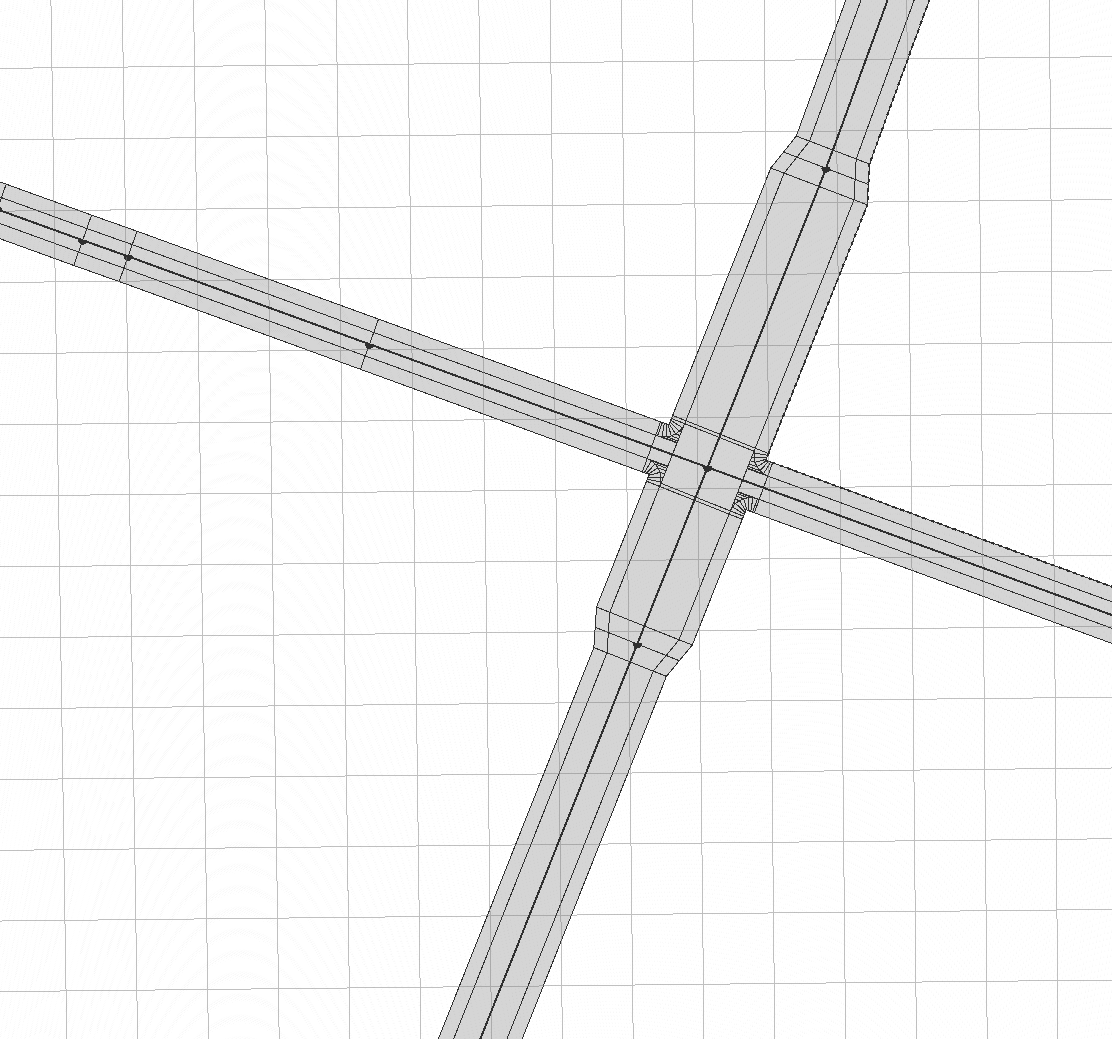
\includegraphics[width=0.4\textwidth]{figures/simply}
	  \label{fig:simply}
	}
	\caption{Comparison of the same CityEngine generated shapes from unsanitised and sanitised \emph{OSM} export file.}
\end{figure}

Since the information in the OSM export is only 2D, CE attempts to determine the perfect location for every shape, although most of them overlap. Therefore, it chooses \texttt{y} values which would generate reasonable shapes. Clearly, the scene generated in this way could not be used in Unity, so we have to delete some of the data. This was achieved with a Python 3 script which can be found in \texttt{cityengine-mmk/scripts/osmsanitizer.py}. The script accepts only one input parameter, which is the OSM export file and produces a sanitised version of the same export with the appendix \texttt{-sanitized} in its name. It can be executed in the console as following, assuming we are in the same folder as the script: \texttt{python3 osmsanitizer.py ../data/map.osm}. The resulting file \texttt{map-sanitized.osm} will be again situated in \texttt{cityengine-mmk/data} folder. 

The sanitisation process follows a straightforward whitelisting fashion. Firstly, we have to delete all roads which are not drivable by a vehicle. Additionally, we want to preserve information about buildings and parkings which should be also present in the export. As we know from Chapter~\ref{ch:background}, there are two main objects in OSM which hold information about the infrastructure of the road network: \texttt{way} and \texttt{relation}. According to the OSM documentation\footnote{\url{http://wiki.openstreetmap.org/wiki/Key:highway}}, all streets (\texttt{way} objects) must have a \texttt{highway} tag which marks its type. The valid highway tags are \texttt{motorway}, \texttt{motorway\_link}, \texttt{trunk}, \texttt{trunk\_link}, \texttt{primary}, \texttt{primary\_link}, \texttt{secondary}, \texttt{secondary\_link}, \texttt{tertiary}, \texttt{tertiary\_link}, \texttt{unclassified}, \texttt{residential}, \texttt{living\_street}, \texttt{unsurfaced}. If a \texttt{way} object does not contain a \texttt{highway} tag or the type of the road is not one of the aforementioned fourteen values, then it is deleted. Similarly, we check whether a \texttt{way} object contains a \texttt{building} tag which is set to \texttt{yes} and an \texttt{amenity} tag set to \texttt{parking}. This approach leaves in the OSM export buildings and parkings which coordinates and properties can be later imported in CE.

The sanitiser tries to solve another problem with OSM data, too. Sometimes information about streets, \emph{e.g.} speed limits or number of lanes, could be missing. When this is the case CE and SUMO try to extrapolate this information and suggest some valid values in order to create the resulting models. Unfortunately, it could happen that both softwares provide different values for the same part of the road system. Because we want to integrate the information streams coming from both, CE and SUMO to create a semantic description of the road network, this data extrapolation has to be accomplished one step ahead in the sanitisation process. Therefore, we provide default valid values for possibly missing or damaged information and add it to the OSM objects in the final sanitised file.

Finally, we have an OSM data which is valid and contains only the necessary information to build 3D shapes from it. Note that we do not delete any \texttt{node} objects because unused nodes, \emph{i.e.} not connected by a way or a relationship, are by default discarded in both, CE and SUMO.

\section{Building the Semantic Road Description}
After we have accomplished the sanitisation of the OSM data, we can provide the resulting file to both CityEngine and SUMO as can be seen in Figure~\ref{fig:overview}. Overall, we use the CE's Python interface to traverse all necessary objects and extract their properties. Afterwards, using the OSM ID, we extract lane information about the road network generated by SUMO, which is not available in CE. In the end, the combined information from CE and SUMO is exported as JSON format, which structure is described in Section~\ref{sec:format}. 

\subsection{OSM Data Import Process}
In order to build a 3D urban scene accompanied by a semantic description of the road network, the user has to execute the steps which will be described in this section. Some of the steps were not able to be automated because of limitations related to CE's Python interface. After starting a CE instance and opening the \texttt{cityengine-mmk} project which contains some essential rules to generate the 3D models, the user has to create a new empty scene. The sanitised OSM file has to be situated in \texttt{cityengine-mmk$\backslash$data} folder. Now the user can drag the file to the 3D viewport and a similar window as in Figure~\ref{fig:import} will show up. Since we have removed all of the unnecessary objects from the OSM file, we can just select all properties to be imported. Next, we can leave the \emph{Map OSM tags} selected, because we will need them later in the export process. Although our sanitiser has prepared the data, we still need \emph{Run Graph Cleanup Tool after Import} option because sometimes OSM data can be still imprecise. This option will delete unnecessary nodes and segments which overlap each other or are incomplete. Finally, we want CE to generate shapes for the road network, therefore we mark the \emph{Create Street/Intersection Shapes from Graph} option, too. There is a way to import an OSM map data directly with the CE's Python interface using \texttt{CE.importFile} and \texttt{OSMImportSettings}. Unfortunately, it is impossible to select which of the each object's attributes to be imported. Moreover, only some of the attributes are selected by default which is not sufficient for our purposes. In the end, one have to select \emph{Finish} and the software will import the data and generate 3D shapes. An example import of the \emph{TU Viertel} in M\"unchen\footnote{\url{https://www.openstreetmap.org/#map=16/48.1493/11.5678}} can be seen in Figure~\ref{fig:ce-1}.

\begin{figure}[htb]
	\centering
	\subfigure[] {
	  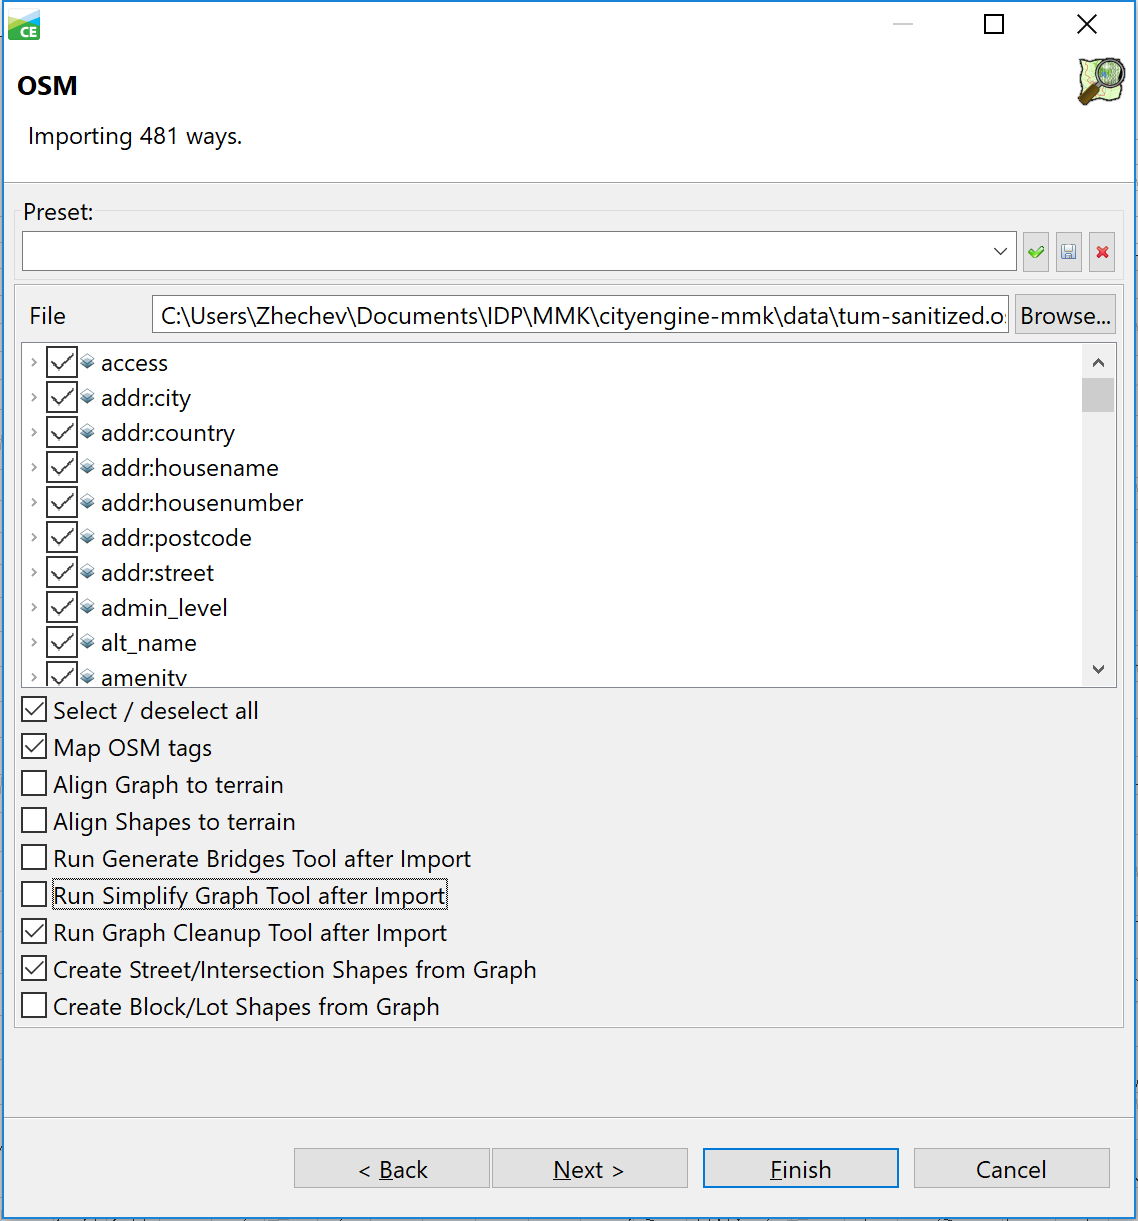
\includegraphics[width=0.28\textwidth]{figures/import}
	  \label{fig:import}
	}%\hspace{0.05\textwidth}% \hfill or \hspace{5mm} or \hspace{0.3\textwidth}
	\subfigure[] {
	  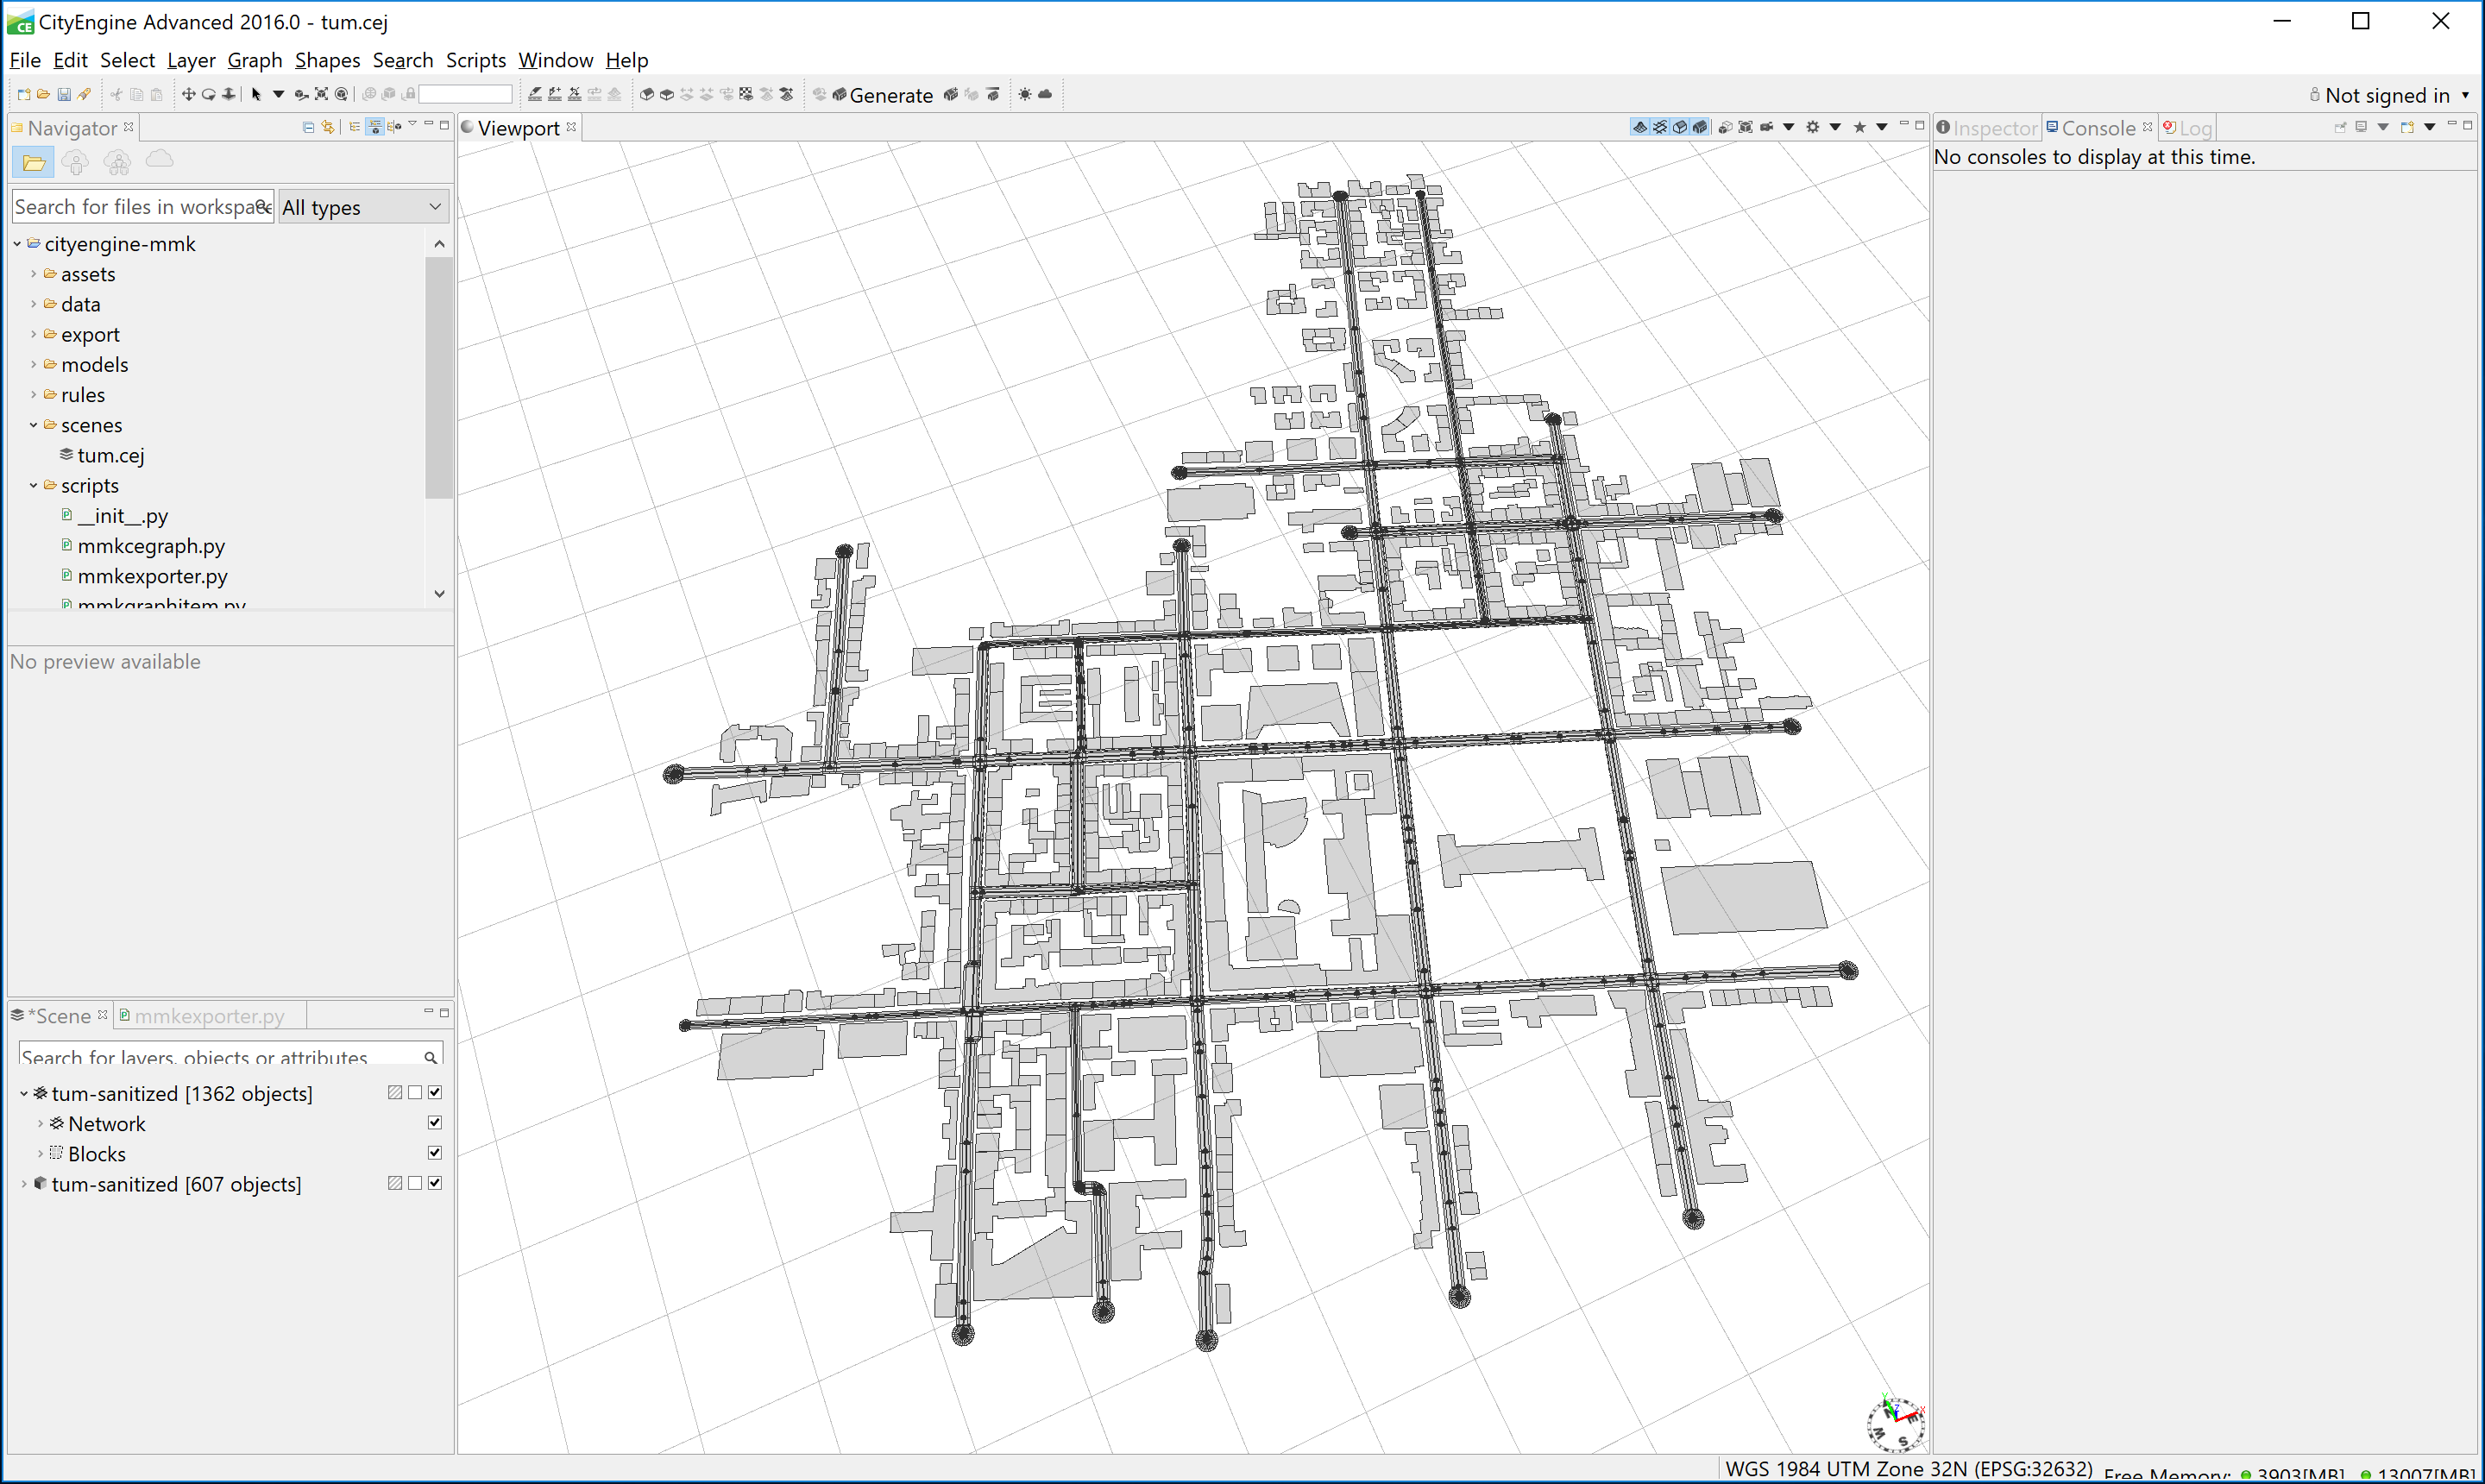
\includegraphics[width=0.68\textwidth]{figures/ce-1}
	  \label{fig:ce-1}
	}
	\caption{Example import dialog of OSM data in CE (a) and the resulting scene (b).}
\end{figure}

\subsection{CE Settings and Way-Segment Inconsistencies}
If we happen to leave the \emph{Run Simplify Graph Tool after Import} option selected, it may alter the imported OSM information, thus making it useless for cross referencing data between OSM and CE. The simplifying strategy of CE tries to merge some neighbouring segments in order to make the underlying road system's shapes more straight. Unfortunately, the CE's algorithm tries to merge properties of segments which are not meant to be combined. If it happens that the two segments, which are going to be combined, posses different OSM ID values, then the new segment receives the arithmetic mean of the two values. Of course, this new ID is not valid and we cannot restore the original segments' IDs which renders it useless. To address this problem, we selected separately segments which have the same OSM IDs and called the simplifying tool only for them. Fortunately, this solved the problem with the destroyed IDs, nonetheless it broke junction's connections. In that case, two ways which were crossing in the middle forming a junction, were separated by CE in 4 segments, one for each exit of the junction. Calling the simplifying tool separately for the two pairs deleted the junction and placed one of the roads above the other by combining the two segments again. Clearly, this was not a solution to this problem, so we decided to unmark this tool since all of the generated shapes until this moment were acceptable.  

Another setting which could negatively influence the shape generation process and therefore decrease the reality of the produced scene is \emph{Run Generate Bridges Tool after Import}. This tool determines whether a segment's \texttt{y} value can be changed so it is lifted above another, underlying structure. This approach introduces some inaccuracies in the generated road models. Since this tool is absent from SUMO (it is only a 2D simulation) and we have to keep the shapes of the two generated urban networks as close as possible, we chose to switch off this option. However, this also means that the user has to furthermore adjust the shapes of some objects to represent the reality while staying coherent with SUMO.

Our first approach to create a semantic description of the road network in CE generated using OSM data involves completely ignoring the imported parameters in CE. We still have to export the vertices of the CE's shapes using the CE's Python interface but all of the information about a given street segment such as number of lanes or speed limits will be directly taken from the OSM export file. The biggest advantage of this approach is that we can accomplish the \texttt{xml}-parsing in Python 3 which might be more performant than using the Jython interface in CE to read all of the attributes. Although this is generally true, we would break the export functionality in two big modules which are highly coherent and they normally belong in one place. Moreover, there was another obstacle which seemed crucial for the success of this approach. CE does place almost (actually this causes yet another problem which will be discussed later in this section) every OSM node on its correct place and uses its original OSM ID, but this is not the case with segments. According to the shape of a given way (which is determined by its nodes), CE decides in how many actual segments to partition it. In other words, it may happen that one \texttt{way} object has more than one corresponding segments in the CE scene. Unfortunately, this introduces unnecessary difficulties in reconstructing a way from its segments which would be later crucial for the lane generation. Therefore, this first approach was abandoned in favour of a script, purely implemented in the CE's Jython environment which depends on the imported attributes in CE from OSM to reconstruct each object's behaviour. 

\subsection{CE Export}
After importing the OSM data in CE as previously explained, the user has to assign rules to every object (\emph{e.g.} buildings, streets) and generate the 3D models. Some minor adjustments, such as moving buildings or placing crossing marks manually, may be necessary in order to fully prepare the scene for an export. Next, we can start the exporting process which is conducted by the \texttt{MMKExporter} class which can be seen in Figure~\ref{fig:ce-overview-uml}. Firstly, we only consider the \texttt{MMKCEGraph}. 

The \texttt{MMKExporter} traverses all \texttt{nodes}, \texttt{segments} and \texttt{shapes} in CE and parses them together with their attributes in the corresponding \texttt{CEGraphItem} objects (Figure~\ref{fig:ce-uml}). Utilising the CE's Python interface (\texttt{ce.getAttribute(item, 'NameOfAttribute')}), it is easy to access all of the essential attributes of each object which were imported from OSM. As you can see in the UML class diagram in Figure~\ref{fig:ce-uml}, we have adopted a simple inheritance hierarchy which allows extendability, \emph{i.e.} adding more CE objects to the export. As already explained in Chapter~\ref{ch:background}, the whole scene has to be exported in the end to some compatible format. Moreover, one have to specify the \texttt{x}, \texttt{y}, and \texttt{z} offsets which will translate all object's coordinates to the origin. We always leave the \texttt{y} to \texttt{0} since this data is interpolated anyways by CE. However, \texttt{x} and \texttt{z} has to be provided as input parameters to \texttt{MMKExporter} as \texttt{ox} and \texttt{oz}. This is necessary, since the parsed object's coordinates has to be also translated in order to stay coherent with the corresponding 3D models. Additionally, the \texttt{x} and \texttt{y} coordinates of each CE object has to be negated (\texttt{180$^{\circ}$} rotation) in order to correspond to the exported 3D models. Finally, the \texttt{exportJson} method can be invoked after the parsing procedure has finished and the semantic description is saved in the \texttt{export} folder of the CE project in JSON format.

\begin{figure}[htb]
	\centering
	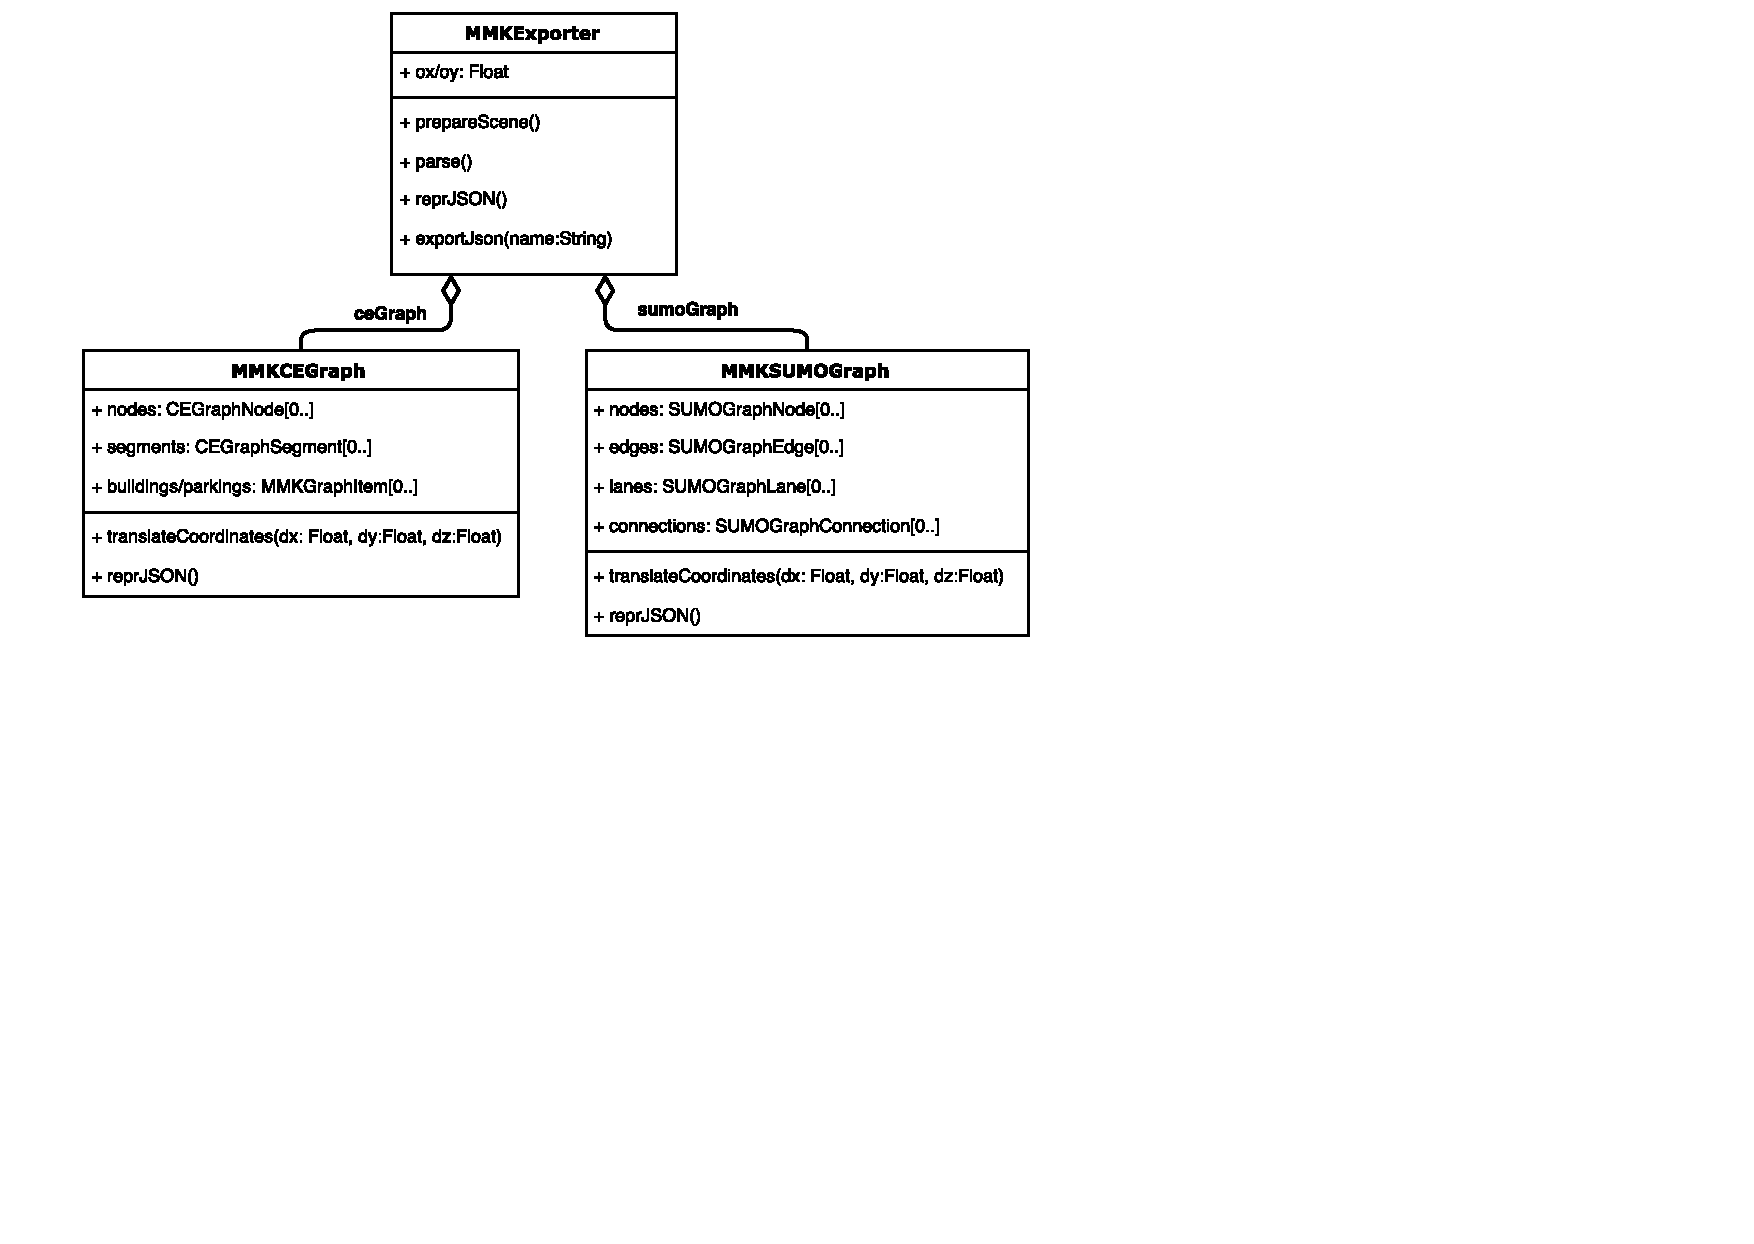
\includegraphics[width=0.65\textwidth]{figures/ce-overview-uml}
	\caption{UML class diagram of \texttt{MMKExporter}, \texttt{MMKCEGraph}, and  \texttt{MMKSUMOGraph}}
	\label{fig:ce-overview-uml}
\end{figure}

\subsection{Additional Information from SUMO}

Now, that we have the basic properties of the road network we can try to extend it with additional data by benefiting from OSM ID values. For instance, we can add lane information and their connectivity to every street segment. Unfortunately, OSM data holds only the number of lanes for each street segment, therefore, CE does not create any lane shapes. We could try to generate lane shapes by interpolating the given data: number of lanes per segment and size of the segment. However, we know that MMK Driving Simulator uses SUMO to simulate other traffic in the scene, which defines its own lane information. Therefore, we can try to synchronise CE and SUMO shapes coordinates and adopt SUMO lanes in our CE export process. This approach was associated with numerous problems which will be discussed in the following.

\begin{figure}[htb]
	\centering
	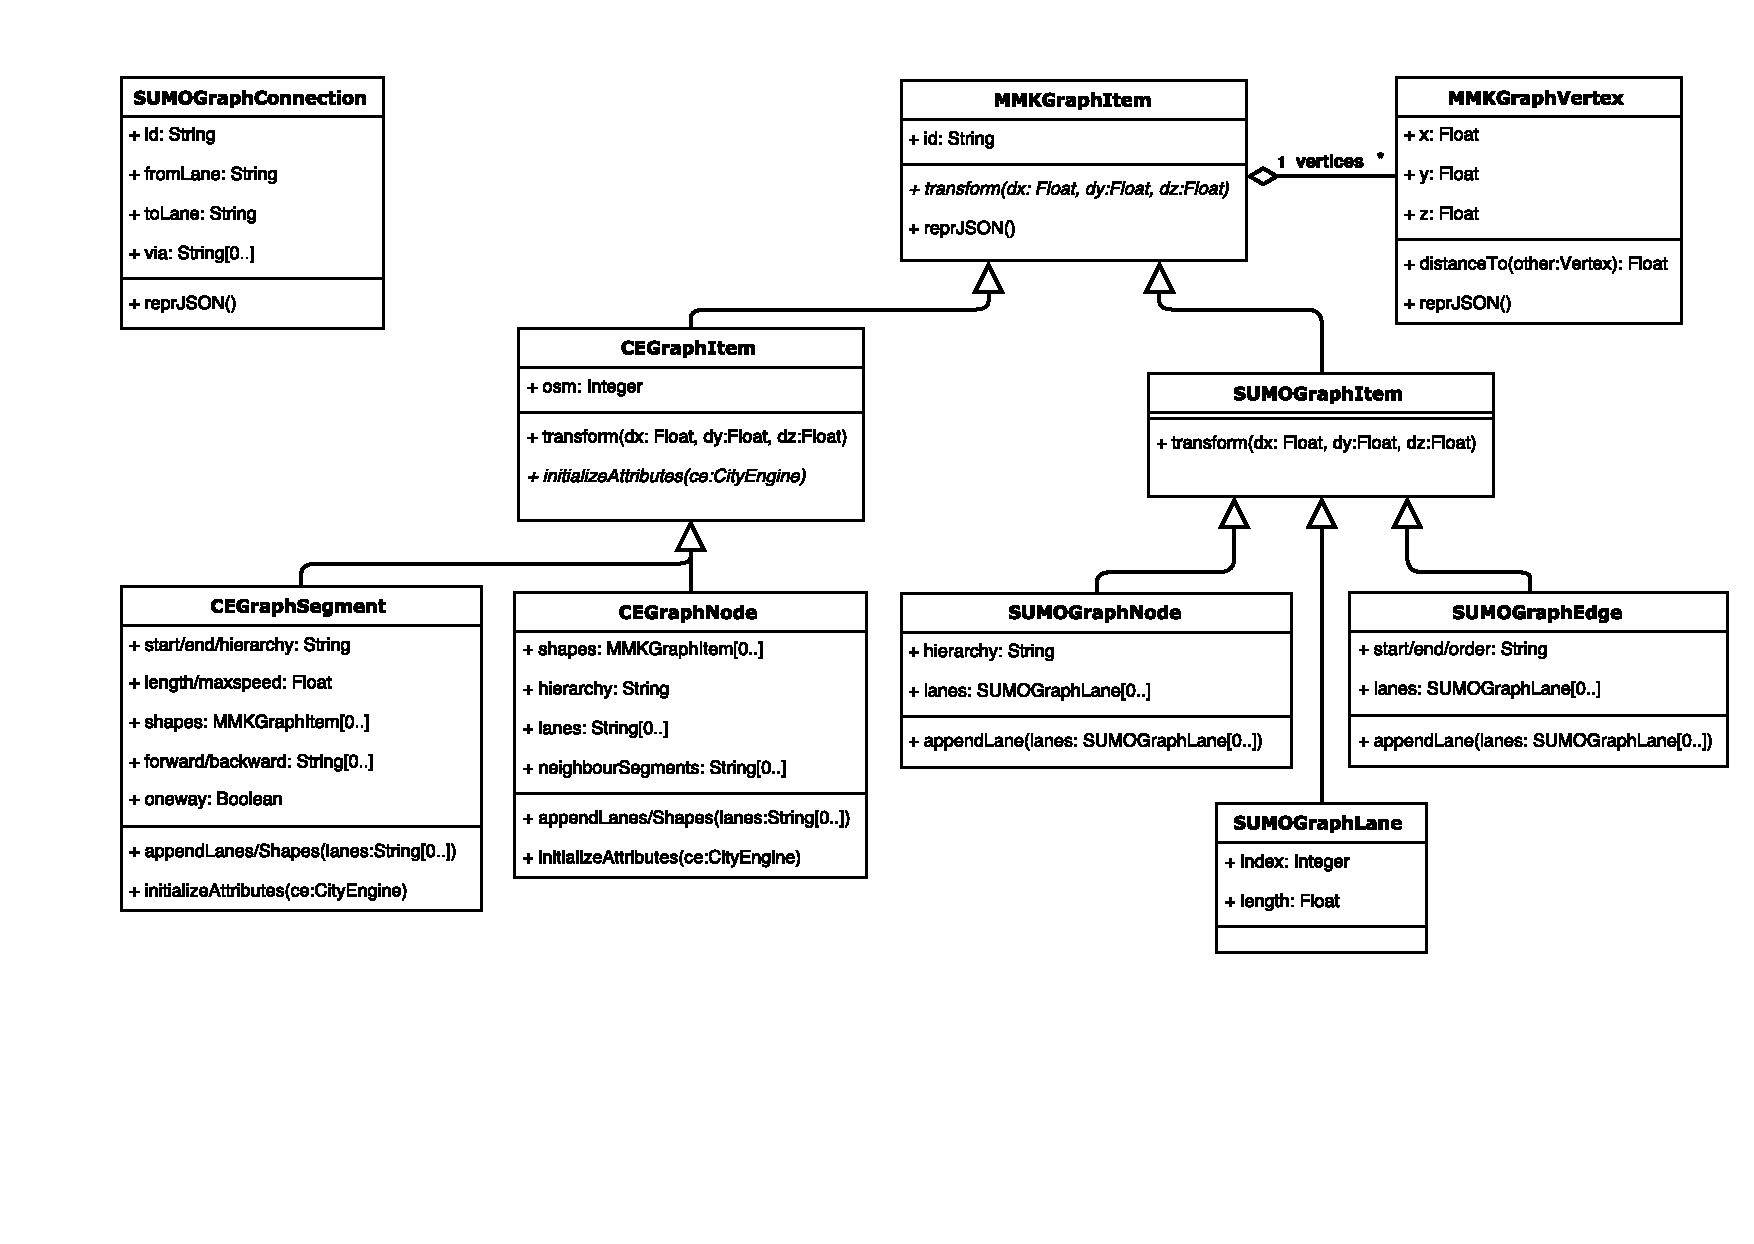
\includegraphics[width=0.9\textwidth]{figures/ce-uml}
	\caption{UML class diagram showing the \texttt{MMKGraphItem} hierarchy and other classes used by the \texttt{MMKExporter}.}
	\label{fig:ce-uml}
\end{figure}

Firstly, we parsed SUMO objects in corresponding \texttt{MMKGraphItem} objects from the \texttt{net.xml} file (Figure~\ref{fig:ce-uml}). We also parsed the connectivity information of the lanes in \texttt{SUMOGraphConnection} objects. As introduced in Chapter~\ref{ch:background}, the imported OSM data in SUMO is projected and translated using some parameters similarly to CE centring export feature. CE and SUMO use the same default projection settings but this is not the case with the translation offsets. Therefore, we had to find these offsets and adjust SUMO object's translation to match the CE configuration. Firstly, it was unknown to us that the \texttt{net.xml} contained a \texttt{location} object which specifies exactly the translation offsets used to adjust all coordinates. Therefore, in order to find the lane's coordinates generated by SUMO in CE's coordinate system, we had to find some correlation between the objects. We know that OSM \texttt{way} objects are sometimes separated in more than one segments in CE. The same is valid for SUMO, so we could not use segments to calculate the necessary translation since more than one segment in CE have the same OSM ID. Then, we decided to take under consideration the nodes which are uniquely identifiable by their OSM ID values in both SUMO and CE. Overall, we searched for the same node in CE and SUMO objects and calculated the difference in their coordinates. These values were then used to translate all SUMO object's coordinates to match CE's models. Moreover, we discovered that SUMO coordinates are rotated by \texttt{180$^{\circ}$} in comparison to CE coordinate system which had to be reversed before translation. This process was accelerated when we started using the offset values defined in \texttt{net.xml}'s node \texttt{location}.

Nonetheless, this was not the only incompatibility between the coordinates of the CE and SUMO objects. Apparently, the algorithms which CE and SUMO employ to generate junctions' shapes have very different features. In Figure~\ref{fig:simply} and Figure~\ref{fig:sumo-incon-1} we can see the same junction created by CE and SUMO. Moreover, Figure~\ref{fig:sumo-incon-2} shows lanes's figures generated by SUMO next to their corresponding CE models. Clearly, SUMO tries to center the streets joining in a junction according to their number of lanes. Since, we cannot interfere in the junction creation algorithms in SUMO and CE, we tried to shift the street models in CE's scene to be alined to SUMO's shapes. This is done in \texttt{prepareScene} method in \texttt{MMKExporter} by adjusting the CE's segments' \texttt{/ce/street/streetOffset} attribute. Firstly, we search for segments which are joining in a junction, then for each segment we subtract its number of forward and backward lanes. The resulting value is then used to shift the current segment either left or right according to its orientation in the whole road network. As already mentioned, OSM \texttt{way} objects can be split into more than one segments in CE and SUMO. Therefore, it could happen that the number of corresponding edges in SUMO and segments in CE is not the same. Thus, one SUMO edge may be represented in CE by two (or more) adjacent segments (from which exactly one is at the junction). Therefore, we have to propagate our shifting algorithm in all directions away from the junction for similar segments, \emph{i.e.} same number and kind of lanes, as well as hierarchy. As a result, we have achieved a cohesion between CE's and SUMO's shape generation process. However, there might be some cases which could not be handled because of the versatile nature of both softwares and the user has to still resolve inconsistencies manually by herself.\\

\begin{figure}[htb]
	\centering
	\subfigure[] {
	  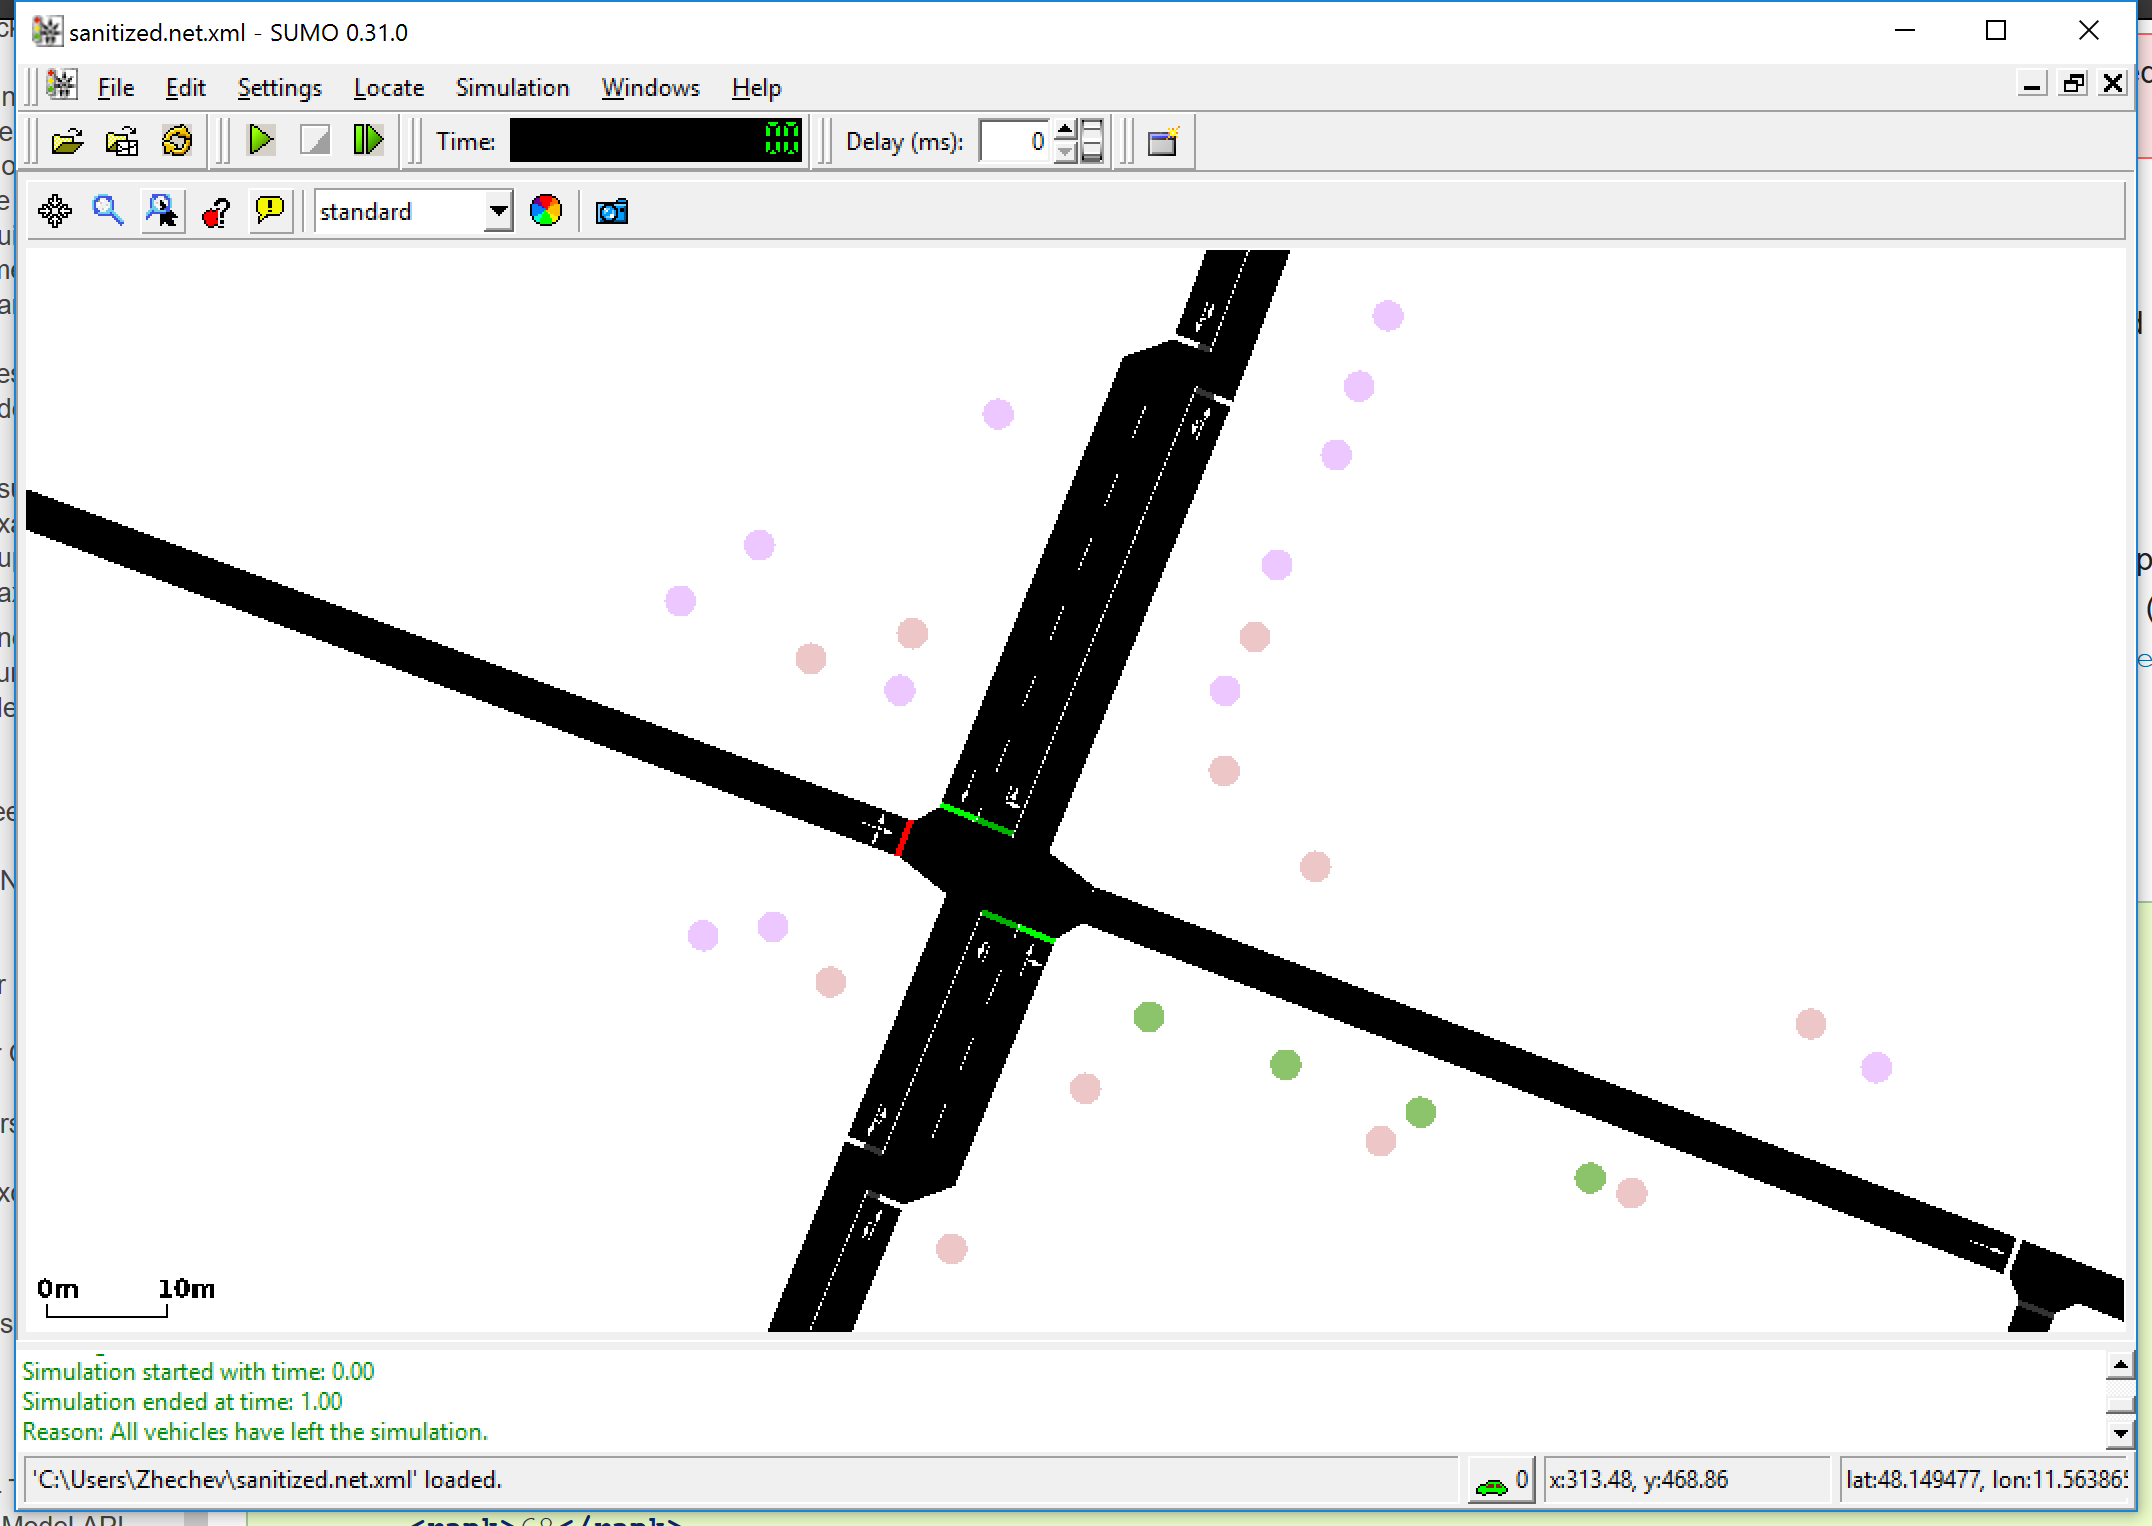
\includegraphics[width=0.4\textwidth]{figures/sumo-incon-1}
	  \label{fig:sumo-incon-1}
	}%\hspace{0.05\textwidth} \hfill or \hspace{5mm} or \hspace{0.3\textwidth}
	\subfigure[] {
	  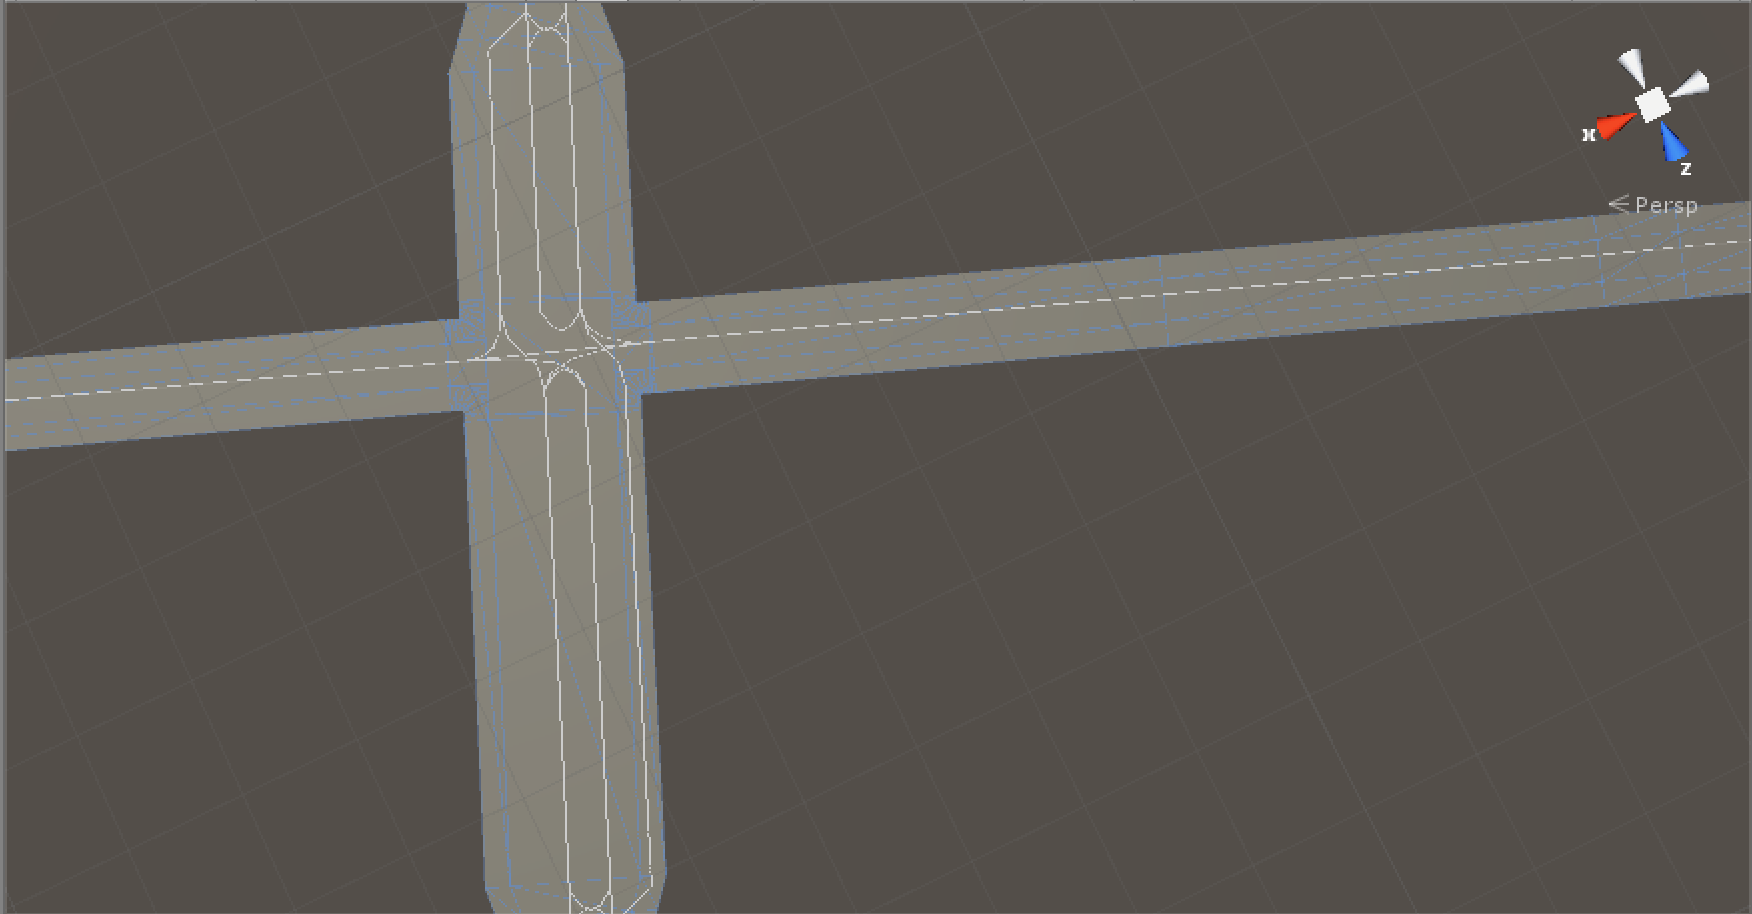
\includegraphics[width=0.5\textwidth]{figures/sumo-incon-2}
	  \label{fig:sumo-incon-2}
	}
	\caption{Inconsistency between SUMO and CE junction creation.}
\end{figure}

Finally, we can start ordering the parsed lanes to their corresponding segments which is only possible because they share the same OSM ID values. We note that in the final format, one lane can be associated to more than one CE segment. However, this ordering process can stumble upon yet another difference between SUMO's and CE's import processes. Even after disabling all shape optimisation routines in CE, it might happen that some nodes are not imported but rather their corresponding segments are attached to another, neighbouring node. We can handle that by looking for nodes which are present in SUMO but missing in CE and finding the nearest existing node in CE. Then, we attach to it the lane's information. However, this operation could be ambiguous because there could be more than one neighbouring nodes. 

In conclusion, we have managed to integrate SUMO generated road information into CE urban network. As a result, we can export this combined semantic road description data as a whole. In the next section we throughly describe the JSON export format which holds this data.

\section{Format Description}
\label{sec:format}
As already introduced, we adopt a JSON format to hold the contents of the semantic description of a road network. In the following, we discuss its advantages and disadvantages, as well as present all essential key value pairs used in the format.

In the beginning of this project, there was an idea to export the street network in OpenDRIVE format which was mentioned in Chapter~\ref{ch:background} in connection to other related work. Although OpenDRIVE allows a precise description of a road network and moreover, it is open-source and can be freely adopted, we withdraw from using it because of synchronisation reasons. More precisely, the data saved in OSM format has to be interpolated~\cite{shi2011automatic}, which would introduce once again another desynchronisation between the road networks built by CE and the SUMO simulation. If this happens, the interpolated lanes in a hypothetical OpenDRIVE format would not coincide with the lane information generated by SUMO. Therefore, SUMO may not be able to be integrated as a simulation environment. Additionally, a JSON format, which we have chosen, has proven to be more human readable and easier to parse. Moreover, there exists a Unity module (Chapter~\ref{ch:background}) which allows easier parsing. A JSON-based format gives us the opportunity to simultaneously provide a thorough description of a certain road network but also adopt and combine other data without breaking their coexistence. 

In Listing~\ref{lis:format-1} one can see a general overview of the used JSON format. Firstly, we define the \texttt{author}, \texttt{date} of the export and the name of the \texttt{project}. These can be also changed in the \texttt{MMKExporter} script to arbitrary values. The more crucial parts of the export are \texttt{nodes} and \texttt{segments}. Obviously, each of these arrays hold all of the nodes, respectively segments in the CE scene. Previously, in the research project by Maximilian Murauer, next to these values, there were also the number of all elements which the both arrays hold. We have chosen to eliminate these values since every parsing process can count the elements in each array. Next, the JSON export contains the \texttt{offsets} of CE and SUMO which were applied to each vertex coordinates in order to compose one coherent scene. Then, we have the \texttt{connections} array which holds all possible links between lanes which is later used to build a navigation system in the next chapter. Lastly, \texttt{sceneObjects} holds vertex information about other objects in the scene which have no direct relation to the road network, \emph{e.g.} buildings, parkings.\\

    \begin{scriptsize}
	   \begin{lstlisting}[language=json,firstnumber=1,caption={General overview of the used JSON format for description of road networks.},label={lis:format-1}]
{
    "author": "TUM - MMK",
    "connections": [(*@$\dots$@*)],
    "date": "2017-11-13",
    "lanes": [(*@$\dots$@*)],
    "nodes": [(*@$\dots$@*)],
    "offsets": {(*@$\dots$@*)},
    "project": "cityengine-mmk",
    "sceneObjects": {(*@$\dots$@*)},
    "segments": [(*@$\dots$@*)]
}
	   \end{lstlisting}
    \end{scriptsize}

A sample \texttt{node} value can be seen in Listing~\ref{lis:format-node}. Firstly, we define its \texttt{hierarchy} which is specified by SUMO and it can be one of the following values: \texttt{unknown}, \texttt{priority} or \texttt{traffic\_light} depending on the kind of node. Secondly, each node holds information about every lane which is part of it. Next, we find two id values in the export: \texttt{id} is the OID value generated by CE and \texttt{osm} is obviously its OSM ID. Each node's neighbouring segments are also referenced in the export by their id values. A node can have zero or more shapes which properties can be found in the \texttt{shapes} array. Additionally, each shape has again two kinds of id values (identical to the node's ids). Finally, the coordinates of each node are kept in the \texttt{vertices} key.\\
 	
    \begin{scriptsize}
        \begin{lstlisting}[language=json,firstnumber=1,caption={General overview of the node key in the JSON exportformat.},label={lis:format-node}]
(*@$\dots$@*)
"nodes": [
    {
        "hierarchy": "priority",
        "id": "40170885-31eb-11b2-8d80-00e8564141ba",
        "lanes": [
            ":21457467_0_0",
            (*@$\dots$@*)
        ],
        "neighbourSegments": [
            "46535ea4-31eb-11b2-8d80-00e8564141ba",
            (*@$\dots$@*)
        ],
        "osm": 21457467,
        "shapes": [
            {
                    "id": "40170885-31eb-11b2-8d80-00e8564141ba:0",
                    "osm": 21457467,
                    "vertices": [
                        {
                            "x": 227.979736328125,
                            "y": -0.0,
                            "z": 109.73065185546875
                        },(*@$\dots$@*)
                    ]
            }
        ],
        "vertices": [
                {
                    "x": 232.09375,
                    "y": -0.0,
                    "z": 106.30369567871094
                }
            ]
        },
        (*@$\dots$@*)
],
(*@$\dots$@*)
	   \end{lstlisting}
    \end{scriptsize}
    
Similarly to nodes, each segment has two id values (OID and OSM ID), as well as analogous \texttt{shapes} key. The \texttt{hierarchy} key provides the type of road defined by OSM and each possible value has been described in Chapter~\ref{ch:background}. Next, segments define in their \texttt{lanes} key the direction of each lane (\texttt{forward} or \texttt{backward}). There are some self-explanatory attributes which are specific to segments such as \texttt{maxspeed}, \texttt{oneway}, \texttt{length}. Additionally, each segment holds a reference to its \texttt{start} and \texttt{end} node. Lastly, there is a \texttt{vertices} array holding a list of 3D polygon points which describe the overall shape of the segment.\\

\begin{scriptsize}
        \begin{lstlisting}[language=json,firstnumber=1,caption={General overview of the segments key in the JSON export format.},label={lis:format-lanes}]
(*@$\dots$@*)
"segments": [
    {
        "end": "4545af7a-31eb-11b2-8d80-00e8564141ba",
        "hierarchy": "tertiary",
        "id": "4545fc94-31eb-11b2-8d80-00e8564141ba",
        "lanes": {
            "backward": [
                "-392069506#0_0"
            ],
            "forward": [
                "392069506#0_0"
            ]
        },
        "length": 27.097801453973258,
        "maxspeed": "50",
        "oneway": false,
        "osm": 392069506,
        "shapes": [(*@$\dots$@*)],
        "start": "43422a00-31eb-11b2-8d80-00e8564141ba",
        "vertices": [(*@$\dots$@*)]
    },
],           
(*@$\dots$@*)
	   \end{lstlisting}
    \end{scriptsize}

Lanes objects' structure is straightforward to describe. They posses an \texttt{id} field where their SUMO generated id is saved. Additionally, they have an index, length and a list of vertices describing their shape.\\
 
\begin{scriptsize}
        \begin{lstlisting}[language=json,firstnumber=1,caption={General overview of the lanes key in the JSON export format.},label={lis:format-node}]
(*@$\dots$@*)
"lanes": [
        {
            "id": ":315667013_8_0",
            "index": "0",
            "length": "7.88",
            "vertices": [
                {
                    "x": 34.27750000000003,
                    "y": 0.0,
                    "z": -110.02389160156247
                },(*@$\dots$@*)
            ]
        },
    ],
(*@$\dots$@*)
	   \end{lstlisting}
    \end{scriptsize}
    
Next, we take under consideration the connection objects. The only information they hold is that there is a connection between two lanes (\texttt{fromLane} to \texttt{toLane}). Since, two lanes might be connected through intermediate links, these links are noted in the \texttt{via} array.\\
    
    \begin{scriptsize}
        \begin{lstlisting}[language=json,firstnumber=1,caption={General overview of the connection key in the JSON export format.},label={lis:format-node}]
(*@$\dots$@*)
"connections": [
        {
            "fromLane": "-155040996_0",
            "id": 0,
            "toLane": "392103894#1_0",
            "via": [
                ":4972221472_0_0"
            ]
        }, (*@$\dots$@*)
    ]
(*@$\dots$@*)
	   \end{lstlisting}
    \end{scriptsize}
    
The scene objects are defined as shapes and have all of their properties as described above. Finally, we consider the \texttt{offsets} key which holds the translation parameters applied to every object from CE and SUMO in order to match both coordinate system. \\

    \begin{scriptsize}
        \begin{lstlisting}[language=json,firstnumber=1,caption={General overview of the offsets key in the JSON export format.},label={lis:format-node}]
(*@$\dots$@*)
"offsets": {
        "ce": {
            "x": -690985,
            "z": 5336220
        },
        "sumo": {
            "x": 605.7575,
            "z": 595.5761083984376
        }
    },
(*@$\dots$@*)
	   \end{lstlisting}
    \end{scriptsize}
    
To summarise, the resulting export file with all of its features described in this section holds the necessary information about a given urban network. In the next section we discuss how this file is imported in Unity.

\section{Unity Import}

Finally, we discuss how the generated 3D models and the corresponding semantic road description are imported and used in a Unity scene as can be seen in Figure~\ref{fig:overview}. We explained in Chapter~\ref{ch:background} how CE exported models are loaded in Unity. The next step involves dragging and dropping the model to the Unity scene. Then, the user has to change the scaling of the street model to \texttt{(100, 100, 100)} and add a \emph{BoxCollider} to the ground of the scene. In the end, \texttt{Network} script has to be attached to the model and \texttt{CarRoadDescriptor} script to \emph{MMKCar}. In \texttt{Network} we have to specify the path to the road description file and in \texttt{CarRoadDescriptor} we have to check the name of the 3D urban model. 

All scripts responsible for the parsing of the road network description file and their communication behaviours are depicted in the UML class diagram in Figure~\ref{fig:unity-uml-1}. Similarly to the export process, there are classes which encapsulate road structures, such as edges (\texttt{NetworkEdge}) and lanes (\texttt{NetworkLane}). \texttt{Network} holds the actual graph and it is responsible for its creation from a JSON format file described in the previous section. Upon creation, to every edge and node a \emph{BoxCollider} is assigned which encapsulates its vertices. This is used in the \texttt{CarRoadDescriptor} for optimisation reasons when calculating the currently occupied lane by the vehicle. In order to determine that, we have to perform costly geometrical calculations involving the current coordinates of the car and \textbf{all} lanes in the scene. Instead of traversing all lanes, we could consider only lanes from the current edge or node where the vehicle is situated. This is achieved by tracking which colliders the vehicle is currently triggering. The \texttt{RoadPosition} method is responsible for determining the current lane and segment of the vehicle.

\begin{figure}[htb]
	\centering
	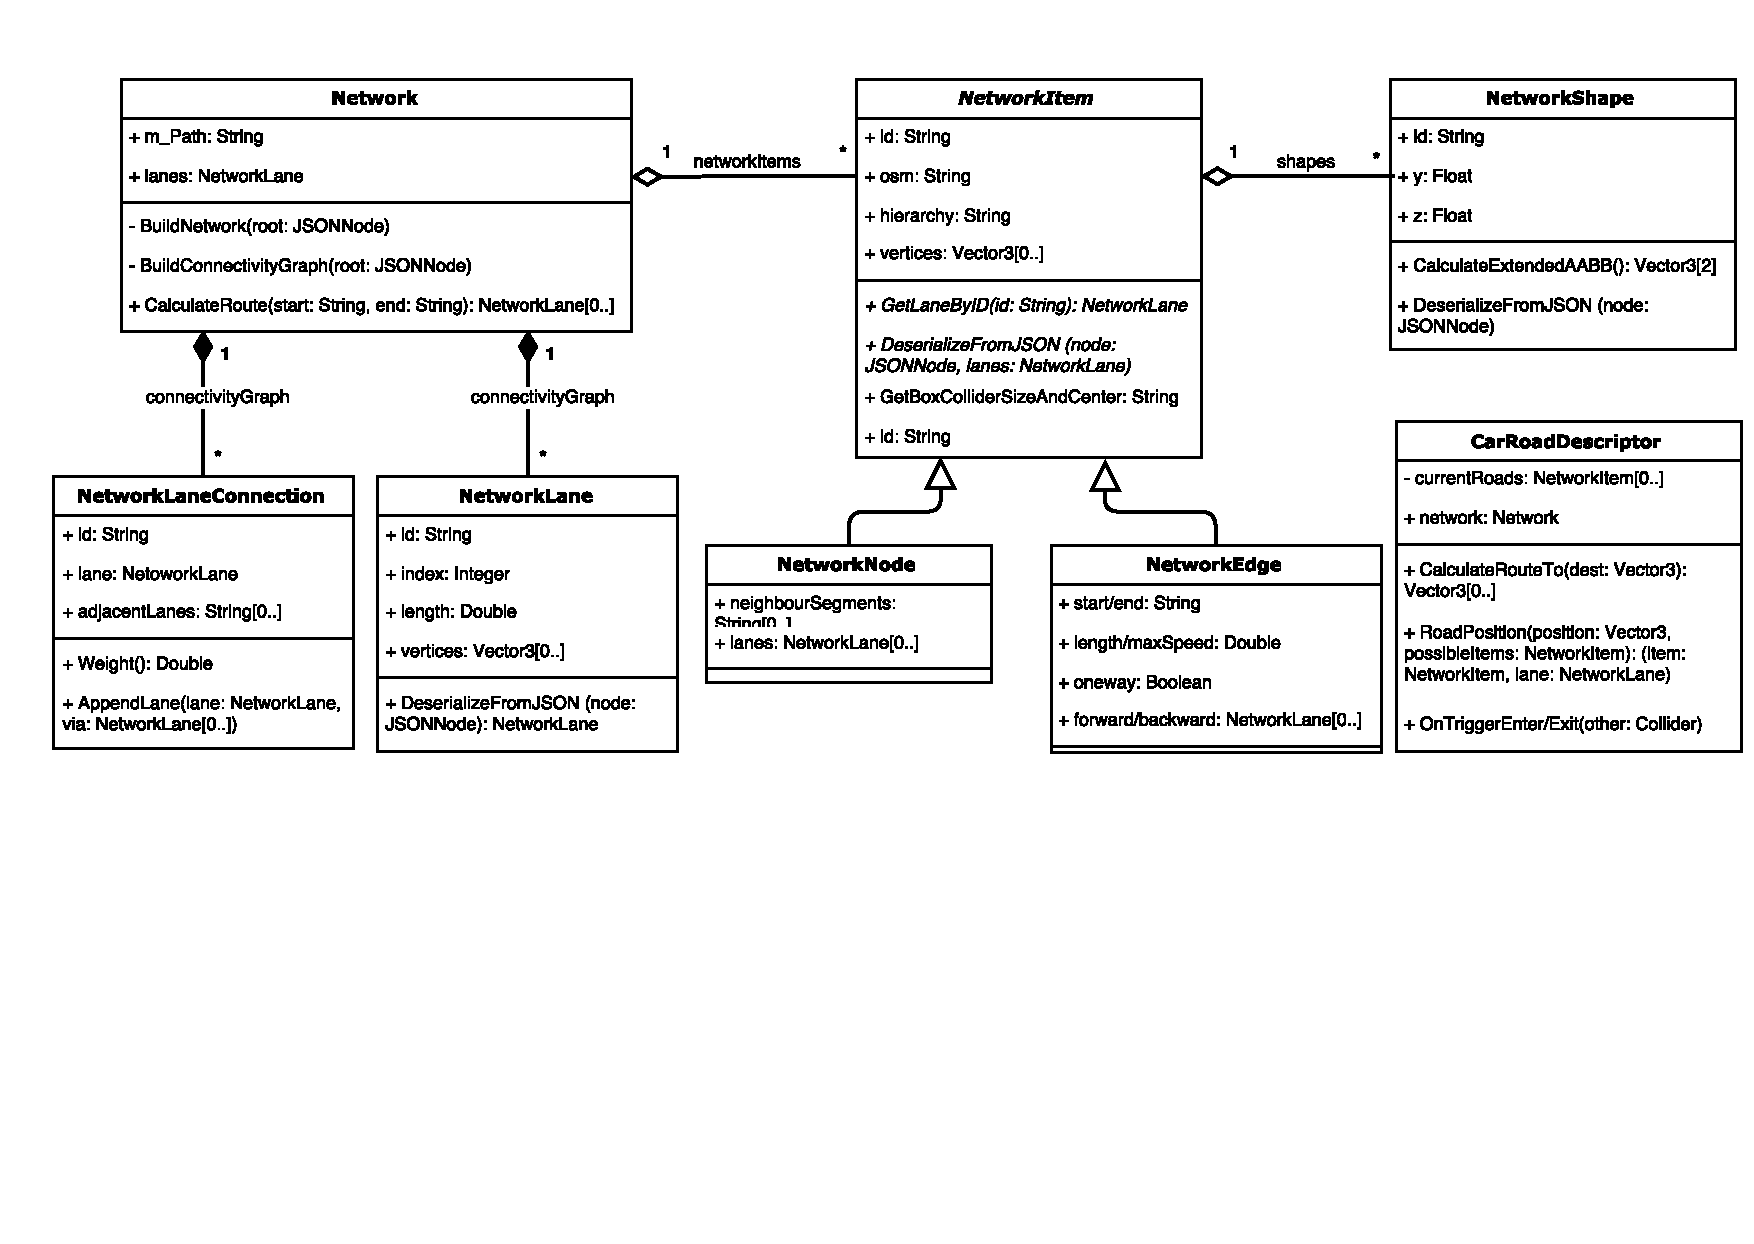
\includegraphics[width=0.9\textwidth]{figures/unity-uml}
	\caption{UML class diagram of modules related to semantic road description in Unity's project.}
	\label{fig:unity-uml-1}
\end{figure}

The whole scene generation process, as well as the semantic road description export have been applied to an OSM export data from different parts of the world. A 3D scene of \emph{TU Viertel} in M\"unchen and the corresponding description of the urban network can be found in the CE project. 



\chapter{Routing}
\label{ch:gps}

There are many applications of the semantic road description which can be used to improve the usability of the MMK Driving Simulator. One such application is navigation which we will discuss in this chapter. In Figure~\ref{fig:nav} one can see a vehicle (above, right) which wants to reach the blue point (down, right). Utilising the connectivity of the lanes derived by SUMO, as explained in the previous chapter, we can calculate the shortest possible path. This path is shown in the figure using red dots. Moreover, one can see that we have included to the path the \texttt{via} lanes, too. In the following, we describe the employed algorithms to calculate an ordered list of points which a vehicle has to follow in order to reach a predefined destination. Additionally, we discuss our design decisions, as well as some limitations which were recognised during development.

\begin{figure}[htb]
	\centering
	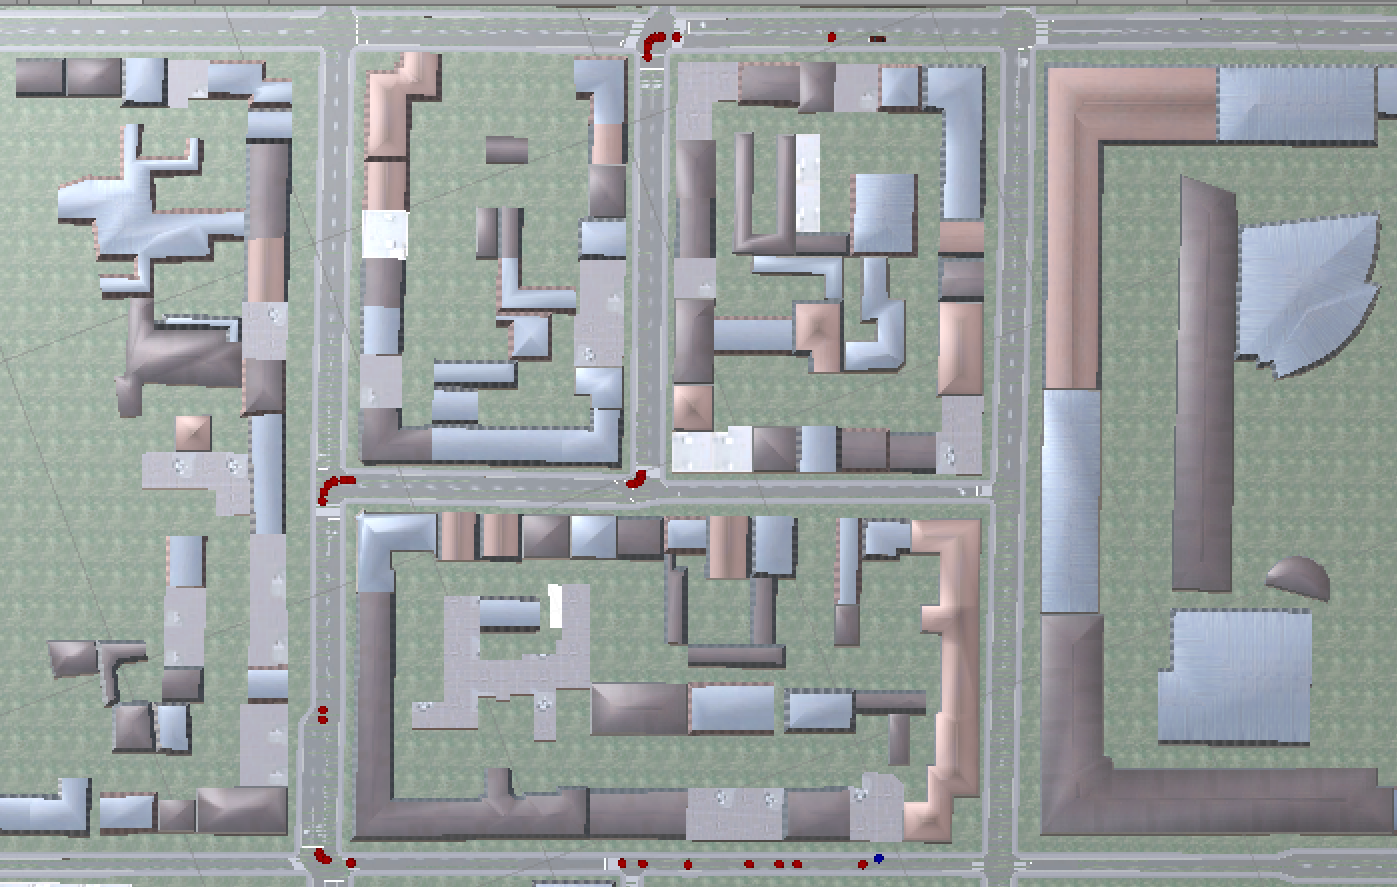
\includegraphics[width=0.9\textwidth]{figures/nav}
	\caption{MMK Car, above right and the calculated shortest path (red) to a predefined user destination (down right, blue).}
	\label{fig:nav}
\end{figure}
\section{Routing Algorithm}
Currently, there exist many algorithms able to calculate the shortest path between two points, \emph{e.g.} Dijkstra, Bellman-Ford, A*. Some of these algorithms work under special conditions, \emph{e.g.} Dijkstra can be applied to graphs where no edge has negative weight. On the other hand Bellman-Ford is more versatile, as it is capable of handling graphs in which some of the edge weights are negative. Since in our graph there are only edges with positive weights, we decided to choose Dijkstra for our implementation.

Dijkstra's algorithm is a shortest-path algorithm that iteratively searches from a start node \emph{s} to a target note \emph{t}~\cite{skiena1998algorithm}. From a currently visited node \emph{v}, all neighbouring, unvisited nodes get a weight set based on the edge weights. Each node encountered gets a weight \emph{w} assigned which denotes the distance from \emph{s} to this node via the current node \emph{v}. If a node already has a weight, it is only changed if the new weight would be lower, ensuring an optimal solution.

The algorithm forms a circle around the start node, with a radius increasing in each step. The search can be stopped once \emph{t} has been visited. The resulting path is the shortest path from \emph{s} to \emph{t}.

\section{Implementation Details}
First of all, we have to build a graph from the provided lane connectivity information in order to apply Dijkstra to it and calculate the shortest path between two points. However, this cannot be done in a straightforward way because in this case the nodes of the graph are the actual lanes and the connections are links between them which have no length. Of course, some connections have "via" lanes which can be used to calculate the distance between two lanes but this cannot be applied everywhere. We note that, in order a vehicle to drive from the start of a given lane A to the start of another, adjacent to A, lane B, it has to drive through the whole lane A. This intuition helped us to design the actual graph. Since links between lanes do not provide weight information (apart from the sum of the length of via lanes if present), we defined \textbf{the weight of an edge} connecting given lane A and lane B (in the direction from lane A to lane B) as the \textbf{length of lane A}. Since, there is no connectivity information for neighbouring lanes, we do not consider these connections.

After designing the graph, we have to decide its representation in memory. There are many possibilities to achieve this, \emph{e.g.} adjacency matrix/array/list, edge list. The most crucial part of the Dijkstra algorithm as already explained is the finding of neighbouring nodes, which has to be done in an efficient way. Therefore, we have chosen to utilise an adjacency list to hold the graph information. Additionally, we implemented a special object \texttt{NetworkLaneConnection} (Figure~\ref{fig:unity-uml-1}). In the \texttt{Network} class, using the \texttt{BuildConnectivityGraph(\_:\;JSONNode)} method we parse all connections defined in the semantic road description export file. Firstly, we initialise a data structure to store all \texttt{NetworkLaneConnection} objects. Each object in this structure has, as can be seen in Figure~\ref{fig:unity-uml-1}, a lane object and a list with all adjacent to it other lanes. Next, for every connection between two lanes, we either create a new \texttt{NetworkLaneConnection} using the \texttt{fromLane} and \texttt{toLane} as respectively the \texttt{lane} attribute and the first lane in the \texttt{adjacentLanes} list. Otherwise, the corresponding \texttt{NetworkLaneConnection} object with the current lane already exists and we just have to store the \texttt{toLane} to the list of adjacent lanes. Additionally, we store all \texttt{via} lanes to the corresponding destination lanes.

Next, we implemented Dijkstra in the \texttt{Network} class which calculates the shortest path between two lanes given their id values. \texttt{SimplePriorityQueue} class presented in Chapter~\ref{ch:background} was utilised to further optimise the algorithm. The id values of the start and destination lane were calculated using the \texttt{RoadPosition} method detailed in Chapter~\ref{ch:descriptionOfRoadSystems}. There are two requirements, which have to be fulfilled in order to execute the algorithm. Firstly, the vehicle has to be on a valid lane and secondly, the destination point has to lay again on a valid lane. Using the id values of the start and destination lane, we can invoke the \texttt{CalculateRoute} method in \texttt{Network} class. The result is a list of \texttt{NetworkLane} objects which has to be traversed in order a vehicle to reach the desired destination, starting from its current location. If there is no route found or some of the aforementioned two requirements are not met, then the method returns \texttt{null}. Nonetheless, this is not the result we expected in the beginning because the vehicle awaits from us an ordered list of navigation points which it can follow.\\

\begin{figure}[htb]
	\centering
	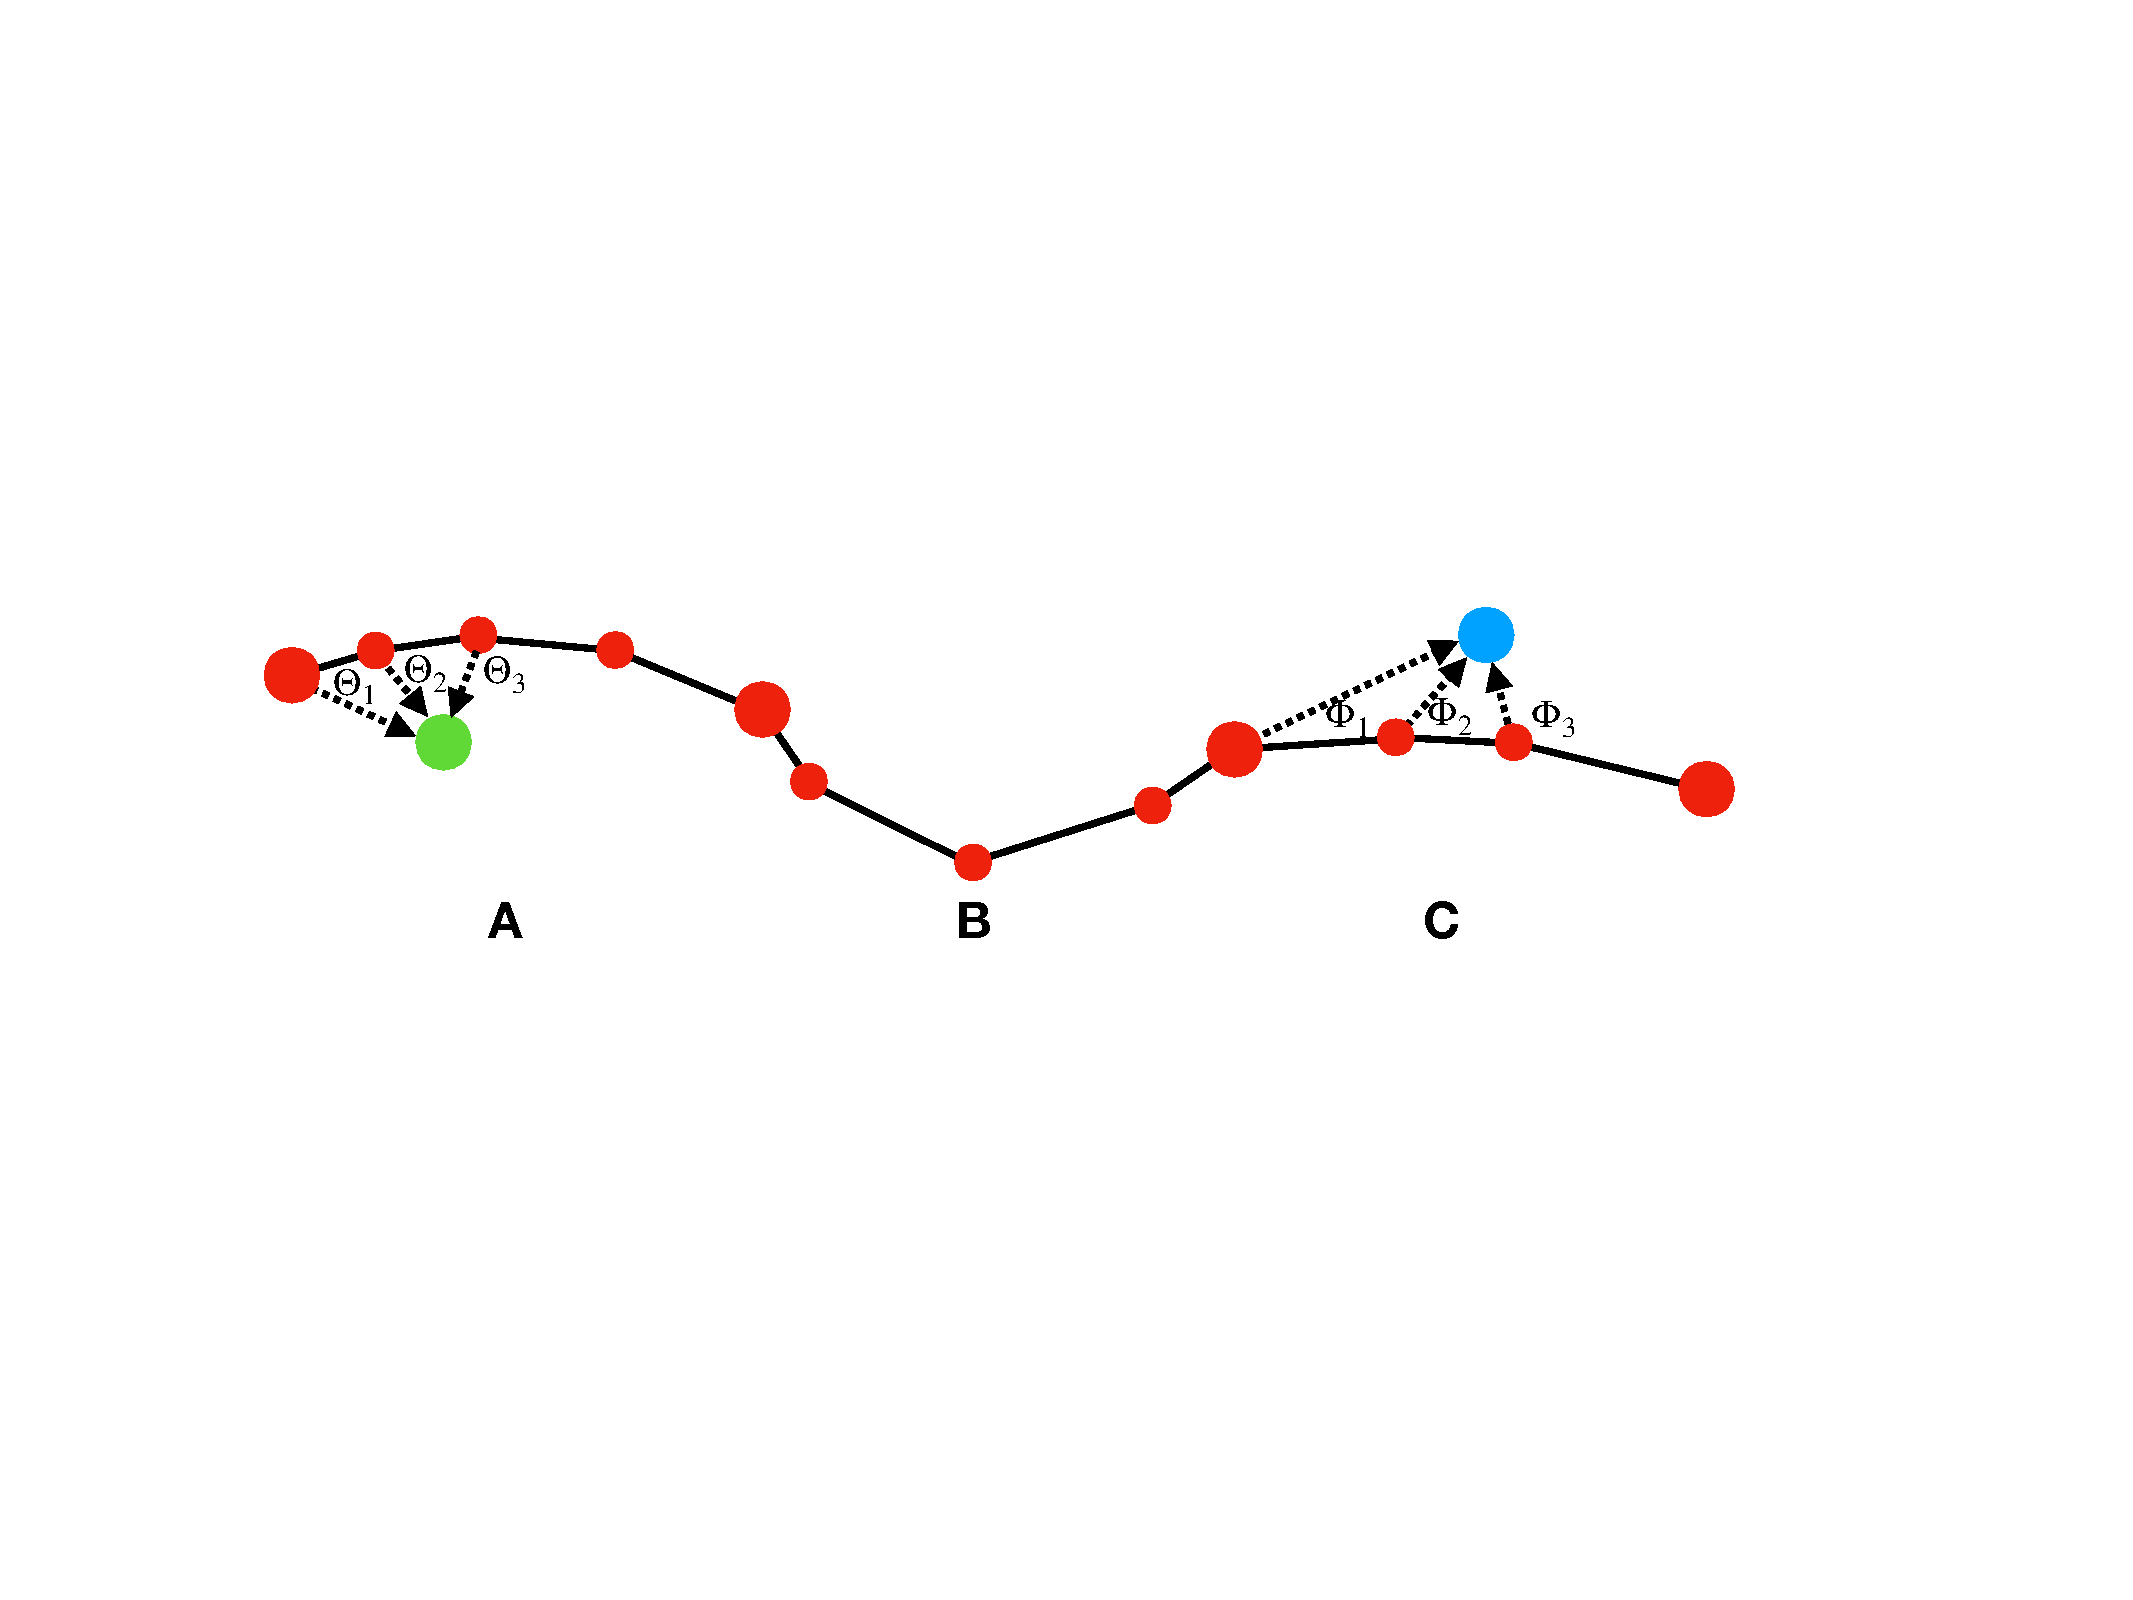
\includegraphics[width=0.9\textwidth]{figures/navpoints}
	\caption{Given a path of lanes (direction from A via B to C) and the coordinates of the vehicle at the start (green point) and the destination (blue point), we use the \emph{dot} product to calculate which points have to be excluded from the final path.}
	\label{fig:navpoints}
\end{figure}

Lastly, we have to collect all points which construct each lane on the calculated shortest path. Generally, there are two cases where lanes have to be handled separately: (1) the first and the last lane, (2) all lanes between them. Since the vehicle does not necessarily start driving through the given route from the start of the first lane, but rather from where it is currently situated, we have to exclude all lane points which are "before" the vehicle. Similarly, all points "after" the destination coordinates have to be discarded from the route. An example is shown in Figure~\ref{fig:navpoints}, where the green point represents the vehicle, while the blue point is the destination. There are three lanes (A, B, and C), which starts and ends are represented by bigger red dots, and each point on every lane is a smaller red dot. As we can see, the vehicle is already situated after the first two points on the start lane, so they don't have to be included in the navigation route. In order to determine which points have to be excluded from the path, we start in the beginning of the first lane and for each point on it we calculate the \emph{dot} product between the vector built by the current point and the vehicle coordinates and the vector built by the current point and the next point on the lane. If the resulting value is negative, \emph{i.e.} the angle between the two vectors is larger than \texttt{90$^{\circ}$} (or smaller than \texttt{-90$^{\circ}$}), then this point is excluded from the list. Analogously, the same operation is performed for the destination coordinates.

To summarise, in this chapter we designed a graph from the lane connectivity information provided by SUMO and implemented a routing algorithm in order to determine the shortest path between a given start and destination. 

% Conlusion and outlook
\chapter{Conclusion and Outlook}
\label{ch:conclusion}

\section{Conclusion}
In this Interdisciplinary Project we have extended the functionality of the MMK Driving Simulator developed at the Institute for Human-Machine Communication, TUM.

Firstly, we developed a JSON format which holds semantic description of a road network. We used this format to describe a 3D urban environment generated in CityEngine adopting OSM data from a chosen areal. In order to achieve this, we employed the Python interface provided by CityEngine and implemented a Python script which exports the properties of the scene. However, this approach was not enough for a complete description of the considered road network. Therefore, we also imported the same OSM data in SUMO and used it to extend the semantic description with data about valid lanes which facilitate the movement of vehicle in the scene. Furthermore, we implemented a interface which imports this description format in Unity and can be utilised for different purposes, \emph{e.g.} navigation. 

Finally, we used the exported semantic description of a road network to  build a navigation functionality for vehicle in Unity. This can be used to calculate the shortest path from one point to another point on the map.

\section{Outlook}

While in this project we have developed way to semantically describe a road network and showed some of its applications, there are many opportunities for extending the scope of this project in the concept of the Driving Simulator remain. This section presents some of these directions and gives some suggestions how they can be achieved. 

First of all, one could use the the buildings vertex information and place colliders in Unity's scene so the car could not drive through them. This could be done for each building or even better one collider could contain more than one building which are in close proximity. Furthermore, the same idea could be used to combine some of the nearly situated colliders which are generated for every road segment. Finally, the road information can be used to implement autonomous vehicles. 


%%%%%%%%%%%%%%
% Backmatter %
%%%%%%%%%%%%%%
%\cleardoublepage
%\begin{appendix}
%\chapter{Upper Bounds on the Expected Error Probability}
\label{ch:appendix}

\section{Recognition Accuracy Rate}



%\end{appendix}
\backmatter % Here, because appendix has still the mainmatter formatting

% Writes only, e.g., "bibliography" on top of those sections
\renewcommand{\chaptermark}[1]{\markboth{#1}{}}
\renewcommand{\sectionmark}[1]{\markright{#1}{}}

  
\cleardoublepage
\addcontentsline{toc}{chapter}{References}
\bibliographystyle{alpha} % Bibliography
% Add your works that are not cited in the text with the \nocite* command


\bibliography{bibliography/thesis}

\end{document}
